\documentclass[12pt,openany]{report}
\usepackage[utf8]{inputenc}
\usepackage[T1]{fontenc}
\usepackage[brazilian]{babel}
\usepackage{geometry}
\geometry{a4paper, top=3cm, bottom=2cm, left=3cm, right=2cm}
\usepackage{graphicx}
\usepackage{amsmath}
\usepackage{amssymb}
\usepackage{booktabs}
\usepackage{tabularx}
\newcolumntype{L}[1]{>{\raggedright\arraybackslash}p{#1}} % coluna de largura fixa alinhada à esquerda
\newcolumntype{Y}{>{\raggedright\arraybackslash}X}  % coluna X alinhada à esquerda
\usepackage{setspace}
\usepackage{indentfirst}
\usepackage{titlesec}
\usepackage{caption}
\usepackage{tikz}

% FONTES COMPATÍVEIS COM A REFERÊNCIA
\usepackage{lmodern}          % Ativa a família Latin Modern
\usepackage{chngcntr}

% MARCAÇÃO DE PENDÊNCIAS (TODOs) DURANTE A REDAÇÃO DO TG2
% Para a versão final: trocar a opção por [disable] para sumir com todos os TODOs.
\usepackage[dvipsnames]{xcolor}
\usepackage[textsize=small]{todonotes}
\setlength{\marginparwidth}{1.8cm}
\newcommand{\pendente}[1]{\todo[inline,color=Goldenrod!25,bordercolor=Goldenrod]{\textbf{TODO:} #1}}
\newcommand{\inseririmagem}[1]{\todo[inline,color=red!12,bordercolor=red!70!black]{\textbf{\color{red!70!black}$\blacktriangleright$ INSERIR IMAGEM:} #1}}

% CONFIGURAÇÃO DE LINKS INTERATIVOS NO SUMÁRIO
\usepackage[hidelinks]{hyperref} % Cria os links clicáveis e remove as caixas coloridas

% Configurações de espaçamento e parágrafos
\onehalfspacing
\setlength{\parindent}{1.25cm}

% REESTRUTURAÇÃO DOS TÍTULOS
\titleformat{\chapter}[hang]{\normalfont\fontfamily{lmr}\selectfont\Huge\bfseries}{\thechapter\quad}{0pt}{}
\titleformat{\section}{\normalfont\fontfamily{lmr}\selectfont\Large\bfseries}{\thesection\quad}{0pt}{}

\begin{document}

% ==============================================================================
% PAGINA 1: CAPA (Formatada dentro das margens e bordas do ITA)
% ==============================================================================
\begin{titlepage}
    \begin{tikzpicture}[remember picture, overlay]
        \draw[line width = 1.2pt]
            ([shift={(20mm,-20mm)}]current page.north west)
            rectangle
            ([shift={(-20mm,20mm)}]current page.south east);
    \end{tikzpicture}

    \centering
    \vspace*{0.1cm}

    {\large\bfseries INSTITUTO TECNOLÓGICO DE AERONÁUTICA\par}

    \vspace{2.0cm}

    % Logo: coloque o arquivo em TG2/Imagens/ita-logo.png (enquanto não existir, aparece uma caixa no lugar)
    \IfFileExists{Imagens/ita-logo.png}{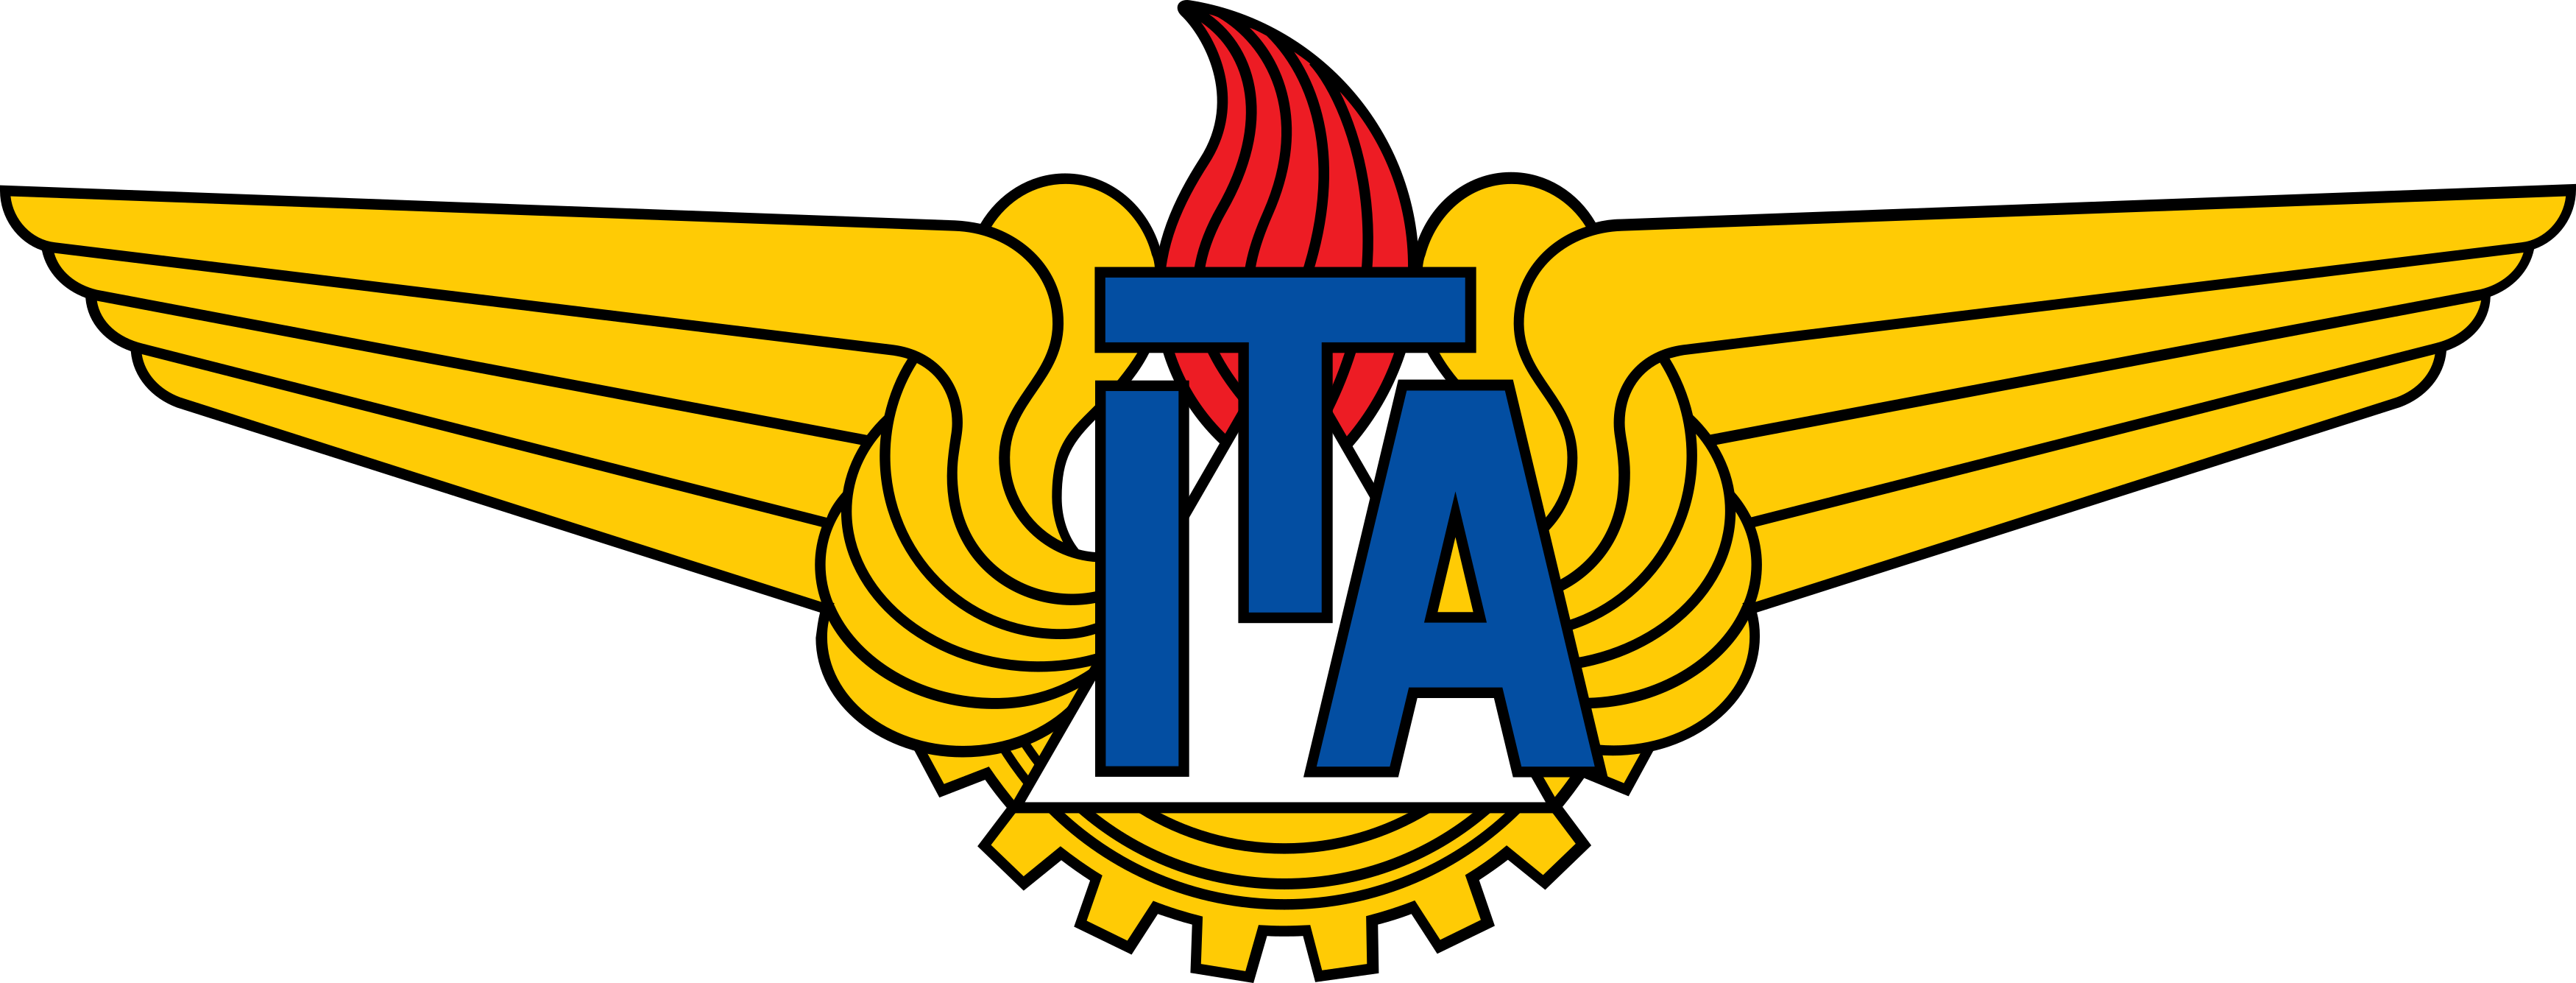
\includegraphics[width=8.2cm]{Imagens/ita-logo.png}}{\fbox{\parbox[c][2.5cm][c]{8.2cm}{\centering [logo ITA --- \texttt{Imagens/ita-logo.png}]}}}\par

    \vspace{2.0cm}
    \begin{singlespace}
        {\Large Rafael Lucas de Albuquerque Louvain \par}
    \end{singlespace}

    \vspace{2.0cm}

    \begin{minipage}{\textwidth}
        \centering
        {\Large\bfseries
        ANÁLISE DA INFLUÊNCIA DE PARÂMETROS DE PROCESSO DE FABRICAÇÃO (CINEMÁTICOS, DE GEOMETRIA DA FERRAMENTA, ENTRE OUTROS) NA INTEGRIDADE DE JUNTAS SOLDADAS POR FSW\par}
    \end{minipage}

    \vspace{2.2cm}

    \begin{singlespace}
        {\Large Trabalho de Graduação \par}
        {\Large 2026\par}

        \vspace{2.8cm}

        {\Large\bfseries Curso de Engenharia Mecânica-Aeronáutica\par}
    \end{singlespace}
    \vspace*{0.2cm}
\end{titlepage}

\newpage

% ==============================================================================
% PAGINA 2: RESUMO
% ==============================================================================
\thispagestyle{empty}
\vspace*{2.5cm}

\begin{center}
    {\fontfamily{lmr}\selectfont\Huge Resumo\par}
\end{center}

\vspace{1.8cm}

Este Trabalho de Graduação propõe o desenvolvimento de um modelo matemático-fenomenológico na forma de um Coeficiente Analítico de Vazio ($C_{void}$) para prever de maneira expedita a ocorrência de descontinuidades volumétricas (\textit{voids}) no processo de \textit{Friction Stir Welding} (FSW). A metodologia baseia-se no isolamento e acoplamento de leis físicas fundamentais para agrupar parâmetros independentes de naturezas distintas (cinemática, geométrica, dinâmica, térmica) em uma expressão multiplicativa adimensional única. O objetivo geral consiste em calibrar e validar essa formulação analítica utilizando o conjunto de dados experimentais estáveis de 108 ensaios das ligas aeroespaciais AA2024, AA2219 e AA6061 estabelecido pelo estudo de Du, Mukherjee e DebRoy (2019), publicado na \textit{npj Computational Materials}, periódico do grupo \textit{Nature}. Como objetivo específico, busca-se mitigar a dependência de simulações numéricas pesadas no chão de fábrica, estabelecendo para o índice analítico a meta de superar o patamar de 70\% de acurácia preditiva global em testes cegos, além de estruturar uma hierarquia de sensibilidade fenomenológica das variáveis governantes.

\vspace{1.0cm}
\noindent \textbf{Palavras-chave:} FSW, Coeficiente Analítico, Vazios, Ligas Aeronáuticas, Análise Dimensional.

\newpage

% ==============================================================================
% PAGINA 3: SUMÁRIO
% ==============================================================================
\thispagestyle{empty}
\begin{center}
    {\fontfamily{lmr}\selectfont\Huge Sumário\par}
\end{center}
\vspace{1.5cm}

\begin{singlespace}
\makeatletter
\@starttoc{toc}
\makeatother
\end{singlespace}

\newpage
\pagenumbering{arabic}
\setcounter{page}{4}

% ==============================================================================
% CAPÍTULO 1 - INTRODUÇÃO E CONTEXTUALIZAÇÃO
% ==============================================================================
\chapter{Introdução e contextualização}

A soldagem por fricção e mistura mecânica (\textit{Friction Stir Welding} -- FSW) foi desenvolvida no \textit{The Welding Institute} (TWI), no Reino Unido, em 1991, como uma técnica de união no estado sólido aplicada inicialmente às ligas de alumínio de aplicação aerospacial historicamente classificadas como não-soldáveis por métodos tradicionais de fusão, como as séries 2XXX e 7XXX (MISHRA; MA, 2005). O FSW opera inteiramente abaixo da temperatura de fusão ($T < T_m$), utilizando uma ferramenta rotativa não consumível, composta por um ombro e um pino, inserida na linha de junta entre as chapas e deslocada ao longo dela. A ferramenta desempenha duas funções: aquecer localmente a peça, por atrito entre ferramenta e material e por deformação plástica, e movimentar o material, que atinge o estado viscoplástico, da frente para a parte de trás do pino, onde a junta é consolidada.  A intensa deformação plástica a temperatura elevada produz grãos finos e equiaxiais recristalizados na região soldada, o que confere às juntas boas propriedades mecânicas.


A relevância do FSW para a engenharia aeronáutica decorre da sua aplicação na solda de fuselagens, asas e outras estruturas que utilizam ligas de alta resistência, como as séries de liga de alumínio mencionadas. A dificuldade de soldar esses materiais com métodos mais usuais se dá em razão da microestrutura de solidificação deficiente, da porosidade na zona fundida e da perda significativa de propriedades mecânicas em relação ao material de base; por isso, a união de estruturas aeroespaciais tem sido feita tradicionalmente por rebitagem, com maior complexidade e custo de fabricação. O FSW contorna essas limitações ao operar inteiramente no estado sólido e já foi adotado em aplicações como os revestimentos e a estrutura da aeronave Eclipse 500, os tanques do foguete Delta, estruturas internas do C-17, da Boeing (MISHRA; MA, 2005), e em diversas outras aplicações nos setores aerospacial, naval e automotivo. Além disso, uma característica interessante do FSW é o seu caráter substancialmente mais sustentável em relação às soldagens tradicionais. Isso se dá por três razões principais, são elas: a não necessidade de metal de adição altamente utilizado em ligas soldadas por fusão, o que reduz a demanda por metais auxiliares no processo de solda e poupa significativa quantidade da energia demandada, haja vista a alta demanda energética na produção de materiais metálicos semi-processados de um modo geral, como os arames e varetas usados como metais auxiliares; não geração de gases tóxicos proveninetes da vaporização desses elementos da liga; e, por fim, um ganho na economica energética decorrente de não necessitar superar o calor latente dos metais da liga, que acabam sendo dissipados em métodos tradicionais de soldagem por radiação e condução (MISHRA; MA, 2005).


Apesar dessas vantagens, o sucesso do FSW depende da confluência de diversos fenômenos físicos complexos que governam a distribuição tridimensional de temperatura, as velocidades do material plastificado e as taxas de deformação na região da ferramenta. Alterações nesses campos podem levar à formação de vazios (\textit{voids}) na junta, tipicamente próximos à ponta do pino, que prejudicam tanto as propriedades mecânicas quanto a vida em serviço do componente. Esses defeitos volumétricos são internos e, em geral, identificados por cortes transversais do cordão ou por ensaios não destrutivos, como ultrassom e radiografia. Atribui-se sua origem ao escoamento inadequado e descontínuo do material plastificado ao redor do pino, decorrente, por exemplo, de aporte térmico insuficiente devido a uma rotação baixa para a velocidade de avanço adotada, de um diâmetro de ombro inadequado ou de uma espessura de chapa elevada. A literatura também associa a ausência de vazios a temperaturas de pico entre 80\% e 90\% da temperatura \textit{solidus} da liga (QIAN et al., 2013 \textit{apud} DU; MUKHERJEE; DEBROY, 2019). Ainda assim, apesar dos avanços na identificação das variáveis relevantes, nenhuma explicação mecanística rigorosa nem um critério para a formação de vazios foi estabelecido até o momento (DU; MUKHERJEE; DEBROY, 2019).

Modelos numéricos abrangentes do processo resolvem as equações de conservação de massa, quantidade de movimento e energia para obter os campos tridimensionais de temperatura e velocidade, a taxa de deformação, a tensão de cisalhamento no pino e o torque, exigindo, contudo, considerável esforço computacional. Simulações desse tipo envolvem o acoplamento de modelos térmicos, de dinâmica dos fluidos computacional (CFD) e termomecânicos, com malhas refinadas que chegam a elementos de 0,05~mm na interface entre ferramenta e peça (LASKA et al., 2023). Como alternativa, Du, Mukherjee e DebRoy (2019) aplicaram aprendizado de máquina a um banco de 108 ensaios da literatura: uma rede neural alimentada apenas pelos parâmetros de soldagem, pela geometria da ferramenta e da chapa e pelas propriedades do material, dados normalmente medidos e registrados no chão de fábrica, atingiu 83,3\% de acurácia na predição de vazios; ao substituir essas entradas por variáveis causais (temperatura, taxa de deformação, torque e tensão de cisalhamento máxima no pino) calculadas por modelos mecanísticos, a acurácia subiu para até 96,6\%, ao custo de exigir simulações prévias para cada condição. Em ambos os casos, o resultado é um classificador sem uma relação explícita entre as variáveis de processo e a formação do defeito. Os próprios autores observam que, em sistemas complexos, o comportamento é frequentemente mais bem descrito por um grupo de variáveis do que pelas variáveis individuais, como no caso do número de Reynolds, que caracteriza o regime de escoamento em um tubo melhor do que o diâmetro, a velocidade, a densidade e a viscosidade tomados isoladamente (DU; MUKHERJEE; DEBROY, 2019). Essa observação motiva a busca por um índice que contemple os parâmetros de processo de forma a capturar a complexidade que induz a formação de vazios de forma mais direta durante a definição dos parâmetros de soldagem.

\pendente{\textbf{TGs anteriores do ITA sobre o tema} (pedido do orientador). Levantar trabalhos de graduação, dissertações e teses do ITA sobre FSW/defeitos/modelagem e posicionar este trabalho em relação a eles (1 parágrafo ou subseção ``Trabalhos anteriores no ITA''). \textbf{Bloqueio:} biblioteca/repositório do ITA fora do ar. Já conhecidos: BEZERRA, Â. C. S. (2025), TG, \textit{Análise da energia efetiva por comprimento e ocorrência de defeitos no processo FSW} (registro DCTA/ITA/TC-065/2025); FILHO, J. A. P. C. (2018), dissertação de mestrado, \textit{Análise de integridade estrutural de uma junta tipo topo soldada em liga de alumínio Alclad AA2024-T3 por FSW na indústria aeroespacial}. Buscar também: ``friction stir'', ``soldagem por fricção e mistura'', ``FSW'' no acervo do ITA; perguntar ao Prof. Lindolfo por outros orientados.}

No ITA, o tema foi abordado recentemente por Bezerra (2025), que desenvolveu um modelo termomecânico analítico para estimar a energia efetiva por unidade de comprimento de solda e correlacioná-la, por regressão logística, com a ocorrência de defeitos em juntas de AA2024-T3 a partir dos ensaios de Filho (2018 \textit{apud} BEZERRA, 2025). O autor concluiu que nenhum patamar único de energia mantém todos os defeitos simultaneamente abaixo de 50\% de probabilidade, indicando que a energia linear isolada não é suficiente e que outros parâmetros, como a força axial, também devem ser considerados. O presente trabalho dá continuidade a essa linha ao propor um índice que combine, de forma explícita, variáveis de naturezas distintas.

\section{Objetivo}

O objetivo deste trabalho consiste no desenvolvimento de um modelo fenomenológico-matemático unificado, expresso na forma de um Coeficiente Analítico de Vazio ($C_{void}$), fundamentado nos princípios de análise dimensional e mecânica dos processos de fabricação. O índice proposto visa agrupar as leis de potência físicas que governam a iniciação de defeitos volumétricos, substituindo a complexidade de simulações pesadas por uma equação explícita direcionada à uma utilização prática em um contexto de operação industrial. A meta estabelecida busca calibrar e validar o índice frente à base de 108 ensaios experimentais das ligas AA2024, AA2219 e AA6061 de Du, Mukherjee e DebRoy (2019), estipulando-se o alvo mínimo de 70\% de acurácia preditiva global na classificação binária de integridade de juntas soldadas. Adicionalmente, busca-se estabelecer uma hierarquia de sensibilidade que indique quais naturezas de parâmetros (cinemática, geométrica, térmica e dinâmica) exercem maior influência na formação de vazios.

% ==============================================================================
% CAPÍTULO 2 - REVISÃO DA LITERATURA
% ==============================================================================
\chapter{Revisão da literatura}

Este capítulo reúne os fundamentos que sustentam a formulação do índice proposto. Parte-se da descrição do processo e de suas variáveis (Seção 2.1), passando pela geração de calor e pela temperatura atingida na junta (Seção 2.2), pelo escoamento do material ao redor da ferramenta (Seção 2.3) e pela microestrutura resultante (Seção 2.4), até chegar aos defeitos de vazio (Seção 2.5) e à influência individual de cada parâmetro de processo sobre eles (Seção 2.6). Em seguida, apresentam-se as abordagens de modelagem e predição de defeitos existentes, com destaque para o estudo de Du, Mukherjee e DebRoy (2019) que fornece a base de dados deste trabalho (Seção 2.7), e os princípios de análise dimensional que fundamentam a construção de índices adimensionais (Seção 2.8). O capítulo se encerra com uma síntese das implicações dessa revisão para a modelagem (Seção 2.9).

% ------------------------------------------------------------------------------
\section{O Processo FSW: Princípio, Ferramenta e Variáveis}

A soldagem por fricção e mistura mecânica é, em sua essência, um processo de conformação no estado sólido conduzido por uma ferramenta rotativa. Uma ferramenta não consumível, provida de um pino em sua extremidade e de um ombro de diâmetro maior, é posta em rotação e inserida nas bordas adjacentes das chapas até que o ombro toque a superfície da peça; em seguida, a ferramenta é deslocada ao longo da linha de junta. Durante esse percurso, a ferramenta desempenha duas funções: aquecer localmente o material, por atrito e por deformação plástica, e movimentá-lo da frente para a parte de trás do pino, onde a junta é formada sem que haja fusão. Na fase inicial de penetração, o aquecimento vem principalmente do atrito entre o pino e a peça, com alguma contribuição da deformação do material; quando o ombro entra em contato com a peça, o atrito do ombro passa a ser a maior fonte de calor (MISHRA; MA, 2005).

\inseririmagem{Esquema geral do processo FSW (ferramenta, chapas, direção de avanço e de rotação, lados de avanço e de recuo). Opção 1: Mishra e Ma (2005), Fig.~1, p.~2 (``Schematic drawing of friction stir welding''). Opção 2: diagrama próprio. Citar a fonte na legenda.}

A ferramenta é, portanto, o elemento central do processo, e cada uma de suas partes cumpre um papel distinto. O ombro, por sua maior área de contato e maior velocidade periférica, é responsável pela maior parcela do aquecimento e atua também como uma barreira que confina o material aquecido sob a ferramenta, impedindo que ele escape. O pino, por sua vez, é o responsável por cisalhar e movimentar o material ao redor de si, conduzindo-o da frente para a traseira da ferramenta. Do ponto de vista térmico, o tamanho relativo entre pino e ombro é o aspecto mais importante, ao passo que os detalhes do perfil do pino governam principalmente o escoamento do material, a uniformidade da microestrutura e os esforços do processo (MISHRA; MA, 2005).

\inseririmagem{Anatomia da ferramenta (ombro, pino, diâmetros $D$ e $d$). Opções: Mishra e Ma (2005), Fig.~2, p.~3 (``Schematic drawing of the FSW tool''); ou a imagem do slide~5 da apresentação do TG1 (desenho com ``Shoulder'', ``Pin'', $d$ e $D$) e a foto do slide~4 (ferramenta em operação) --- \textbf{identificar a fonte original das imagens dos slides antes de usar}.}

As ferramentas mais difundidas combinam um ombro côncavo com um pino cilíndrico roscado, mas a geometria evoluiu significativamente com o melhor entendimento do escoamento do material. O TWI desenvolveu, por exemplo, os pinos Whorl\texttrademark{} e MX Triflute\texttrademark{}, de formato tronco-cônico, que deslocam cerca de 60\% e 70\% menos material, respectivamente, do que um pino cilíndrico de mesmo diâmetro de raiz. Essas geometrias buscam reduzir a força de soldagem, facilitar o escoamento do material plastificado, favorecer seu transporte para baixo e aumentar a interface entre pino e material, elevando a geração de calor; com elas, chapas de alumínio de até 50~mm de espessura puderam ser soldadas em um único passe. Para juntas sobrepostas, foram desenvolvidos ainda os pinos Flared-Triflute\texttrademark{} e A-skew\texttrademark{}, e os perfis de ombro também passaram a receber ranhuras e cavidades que melhoram o acoplamento com o material (MISHRA; MA, 2005). Revisões mais recentes catalogam uma grande variedade de perfis de pino --- cilíndrico, roscado, cônico, quadrado, triangular, hexagonal ---, com desempenhos que variam conforme a liga e os parâmetros empregados (AHMED; KADHUM; SALLEH, 2024). Apesar dessa evolução, Mishra e Ma (2005) observam que o projeto de ferramentas ainda se baseia em grande parte em conceitos intuitivos e que muitas geometrias são proprietárias, o que dificulta generalizar a influência da ferramenta quando ela não é completamente descrita --- aspecto relevante para este trabalho, cuja base de dados descreve o pino apenas por seus raios na raiz e na ponta.

\inseririmagem{Exemplos de geometrias de ferramenta. Mishra e Ma (2005), Fig.~3, p.~4 (pinos Whorl\texttrademark{} e MX Triflute\texttrademark{}, TWI) e/ou Fig.~6, p.~6 (perfis de ombro vistos por baixo). Opcional: figura de perfis de pino da revisão de Ahmed, Kadhum e Salleh (2024).}

A combinação entre a rotação da ferramenta e seu avanço torna o processo intrinsecamente assimétrico. Define-se como lado de avanço (\textit{advancing side}) aquele em que a velocidade tangencial da ferramenta tem o mesmo sentido da velocidade de avanço, e como lado de recuo (\textit{retreating side}) o lado oposto, em que os dois vetores têm sentidos contrários. Essa assimetria se reflete em praticamente todas as grandezas do processo: a temperatura é ligeiramente maior no lado de avanço (MISHRA; MA, 2005), a zona afetada pelo calor tende a ser mais larga desse lado (LASKA et al., 2023) e, como será discutido adiante, é nele que os vazios costumam se formar.

\inseririmagem{Esquema em vista superior mostrando os lados de avanço e de recuo e o sentido do escoamento ao redor do pino. Opção: imagem do slide~6 da apresentação do TG1 (painéis a--d com linhas de corrente) --- \textbf{identificar a fonte original}; alternativa: diagrama próprio em TikZ.}

Do ponto de vista operacional, os dois parâmetros mais importantes do processo são a rotação da ferramenta, $\omega$, e a velocidade de avanço, $v$. A rotação promove o aquecimento por atrito e a agitação e mistura do material ao redor do pino, enquanto o avanço desloca o material agitado da frente para trás do pino e conduz a solda ao longo da junta. Rotações maiores tendem a gerar temperaturas mais altas e mistura mais intensa, mas esse aumento não é necessariamente monotônico, pois o acoplamento por atrito entre ferramenta e peça varia com a própria temperatura (MISHRA; MA, 2005). A razão entre essas duas velocidades, o avanço por rotação ou \textit{weld pitch} ($v/\omega$), aparece com frequência na literatura como um parâmetro combinado do processo, e será retomada nas próximas seções.

Além das velocidades, três outros parâmetros são decisivos. O primeiro é o ângulo de inclinação da ferramenta (\textit{tilt}), em direção oposta ao avanço, que faz com que o ombro retenha o material agitado pelo pino e o transporte de forma eficiente da frente para trás (MISHRA; MA, 2005) e que gera uma força adicional de forjamento na traseira da ferramenta (MEYGHANI; AWANG, 2022). O segundo é a profundidade de inserção do pino: se for rasa demais, o ombro não toca a superfície original da peça e não consegue movimentar o material, gerando canais internos ou sulcos superficiais; se for funda demais, o ombro afunda na peça, gerando rebarba excessiva e afinamento local da junta (MISHRA; MA, 2005). O terceiro é a força ou pressão axial aplicada, que mantém o contato do ombro com a peça; em máquinas operadas em controle de carga, essa força é ajustada para garantir o contato suficiente do ombro (ALDANONDO et al., 2020). Para materiais de alto ponto de fusão ou alta condutividade, o calor gerado pode ser insuficiente, e recorre-se a pré-aquecimento; para ligas de baixo ponto de fusão, como as de alumínio, pode-se recorrer ao resfriamento para limitar o crescimento de grão e a dissolução de precipitados (MISHRA; MA, 2005).

\inseririmagem{Ângulo de inclinação da ferramenta. Meyghani e Awang (2022), Fig.~1, p.~2 (``exaggeratedly cross-sectional view... while the tilt angle is applied''); ou a imagem do slide~25 da apresentação do TG1 --- \textbf{identificar a fonte original}.}

Quanto à configuração das juntas, as mais usuais são a de topo (\textit{butt}) e a sobreposta (\textit{lap}), a partir das quais se derivam outras, como juntas em T e de canto; em nenhum dos casos é necessária preparação especial das bordas (MISHRA; MA, 2005). Cada configuração apresenta defeitos característicos: em juntas sobrepostas, por exemplo, os defeitos típicos são o \textit{hook} e o \textit{cold lap}, ligados ao escoamento vertical de material na interface entre as chapas, e não vazios volumétricos (ALDANONDO et al., 2020). Existem ainda variantes do processo, como o FSW com ferramenta \textit{bobbin}, que possui dois ombros --- um em cada face da chapa --- e dispensa a placa de apoio, reduzindo drasticamente a força vertical e eliminando defeitos de raiz (AHMED et al., 2021). Este trabalho delimita-se ao FSW convencional de juntas de topo, configuração adotada em todos os ensaios da base de dados utilizada.

\inseririmagem{Configurações de junta. Mishra e Ma (2005), Fig.~7, p.~7 (topo, borda, T, sobreposta, múltipla sobreposta, T sobreposta e filete). Opcional: Ahmed et al. (2021), Fig.~1, p.~4 (esquema do processo com ferramenta \textit{bobbin}).}

% ------------------------------------------------------------------------------
\section{Geração de Calor e Temperatura}

O calor no FSW provém de duas fontes: o atrito entre a ferramenta e a peça e a deformação plástica do material ao redor da ferramenta. Na fase inicial de penetração, o aquecimento resulta principalmente do atrito entre o pino e a peça; quando o ombro entra em contato com a superfície, o atrito do ombro passa a constituir a maior parcela do aquecimento. Além de gerar calor, o ombro confina o volume de material aquecido sob a ferramenta. Do ponto de vista térmico, o tamanho relativo entre pino e ombro é o aspecto geométrico mais importante (MISHRA; MA, 2005).

A contribuição de cada parte da ferramenta pode ser estimada por modelos analíticos. Schmidt et al., conforme revisado por Mishra e Ma (2005), propõem para o calor total gerado a expressão

\begin{equation}
Q_{total} = \frac{2}{3}\pi\left[\delta\,\frac{\sigma_{yield}}{\sqrt{3}} + (1-\delta)\,\mu\,p\right]\omega\left[\left(R_{shoulder}^{3}-R_{probe}^{3}\right)(1+\tan\alpha) + R_{probe}^{3} + 3R_{probe}^{2}H_{probe}\right],
\label{eq:schmidt}
\end{equation}

\noindent em que $\sigma_{yield}$ é o limite de escoamento, $\omega$ a velocidade angular da ferramenta, $R_{shoulder}$ e $R_{probe}$ os raios do ombro e do pino, $\alpha$ o ângulo de cone do ombro, $H_{probe}$ a altura do pino, $p$ a pressão de contato, $\mu$ o coeficiente de atrito e $\delta$ a variável de estado de contato. Para $\delta = 1$ tem-se a condição de adesão plena (\textit{sticking}), em que o calor é governado pela tensão de escoamento do material cisalhado; para $\delta = 0$, a condição de escorregamento (\textit{sliding}), em que o calor decorre do atrito $\mu p$ (MISHRA; MA, 2005). A dependência com o cubo do raio do ombro explica a predominância desse componente no aporte térmico. Ahmed et al. (2021), ao modelar a geração de calor em FSW com ferramenta \textit{bobbin} e pinos cilíndrico, quadrado e triangular, estimaram que os ombros respondem por aproximadamente 78\% a 88\% do calor total, conforme a geometria do pino, e que o calor gerado cresce com a rotação, o coeficiente de atrito, o raio do ombro, a espessura da chapa e a área superficial do pino, sendo inversamente proporcional à velocidade de avanço. Os mesmos autores destacam que o coeficiente de atrito diminui com o aumento da temperatura na interface, variando tipicamente entre 0,4 e 0,5.

\inseririmagem{Contribuição das partes da ferramenta no calor. Opções: Ahmed et al. (2021), Fig.~6, p.~10 (efeito da rotação e da velocidade de avanço no calor gerado por comprimento) e Fig.~7, p.~11 (efeito do raio do ombro e do raio do pino). Alternativa: imagem do slide~16 da apresentação do TG1 --- mas a equação já está no texto; usar figura só se acrescentar informação.}

Uma estimativa mais simples da potência média foi proposta por Frigaard et al., conforme revisado por Mishra e Ma (2005): $q_0 = \frac{4}{3}\pi^{2}\mu P \nu R^{3}$, em que $\mu$ é o coeficiente de atrito, $P$ a pressão, $\nu$ a rotação da ferramenta (em rotações por segundo) e $R$ o raio da ferramenta. Segundo esses autores, a rotação e o raio do ombro são as principais variáveis do processo, e a pressão não pode exceder a tensão de escoamento do material na temperatura de operação se se deseja obter uma solda sã, sem depressões. Medições com termopares confirmam a predominância do ombro: em soldas de AA6061-T6, Tang et al., também revisados por Mishra e Ma (2005), compararam ferramentas com e sem pino e verificaram que o ombro domina a geração de calor, o que atribuíram à maior área de contato, à maior pressão vertical e à maior velocidade linear do ombro em relação ao pino. Os mesmos ensaios mostraram que a temperatura cresce com a rotação e com a pressão de soldagem, mas com ganhos decrescentes: cerca de 40~°C ao passar de 300 para 650~rpm e apenas cerca de 20~°C de 650 para 1000~rpm.

\inseririmagem{Predominância do ombro e efeito da rotação na temperatura de pico. Mishra e Ma (2005), Fig.~14, p.~16 (temperatura de pico com e sem pino --- é provavelmente o gráfico usado no slide~12 da apresentação do TG1) e Fig.~13, p.~16 (efeito da rotação, 300/650/1000~rpm).}

A temperatura atingida durante o processo é o principal elo entre os parâmetros de soldagem e o comportamento do material. Medições com termopares e estimativas a partir da microestrutura indicam temperaturas de pico de 400~°C a 500~°C na zona de mistura de ligas de alumínio, sempre abaixo do ponto de fusão (MISHRA; MA, 2005). Arbegast e Hartley, conforme revisado por Mishra e Ma (2005), relacionaram a temperatura máxima de soldagem a um pseudoíndice de calor $\omega^{2}/v$ na forma

\begin{equation}
\frac{T}{T_m} = K\left(\frac{\omega^{2}}{v \cdot 10^{4}}\right)^{\alpha},
\label{eq:arbegast}
\end{equation}

\noindent com $K$ entre 0,65 e 0,75 e $\alpha$ entre 0,04 e 0,06, em que $T_m$ é a temperatura de fusão da liga. A temperatura máxima observada em diversas ligas de alumínio situa-se entre $0,6\,T_m$ e $0,9\,T_m$, faixa correspondente ao trabalho a quente e, em geral, à solubilização de ligas endurecíveis por precipitação. Segundo os mesmos autores, para uma dada ferramenta e profundidade de penetração, a temperatura máxima é função forte da rotação, enquanto a taxa de aquecimento é função forte da velocidade de avanço; a temperatura é ligeiramente maior no lado de avanço (MISHRA; MA, 2005). Em síntese, a temperatura máxima aumenta com a rotação a velocidade de avanço constante, diminui com o aumento da velocidade de avanço a rotação constante e cresce com a razão entre rotação e avanço; o aumento com a rotação, porém, tende a saturar, pois o coeficiente de atrito na interface varia com a temperatura (MISHRA; MA, 2005). Os próprios autores ressaltam que os diferentes pseudoíndices de calor propostos na literatura têm verificação experimental limitada e não apresentaram tendência geral quando aplicados a conjuntos de dados distintos.

\inseririmagem{Temperatura de pico em função da razão rotação/avanço. Mishra e Ma (2005), Fig.~15, p.~17 (Hashimoto et al.: 2024Al-T6, 5083Al-O e 7075Al-T6).}

Medições em chapas grossas confirmam esse comportamento e acrescentam a variação ao longo da espessura. Em soldas de AA6082-T6 com 32~mm de penetração, Ahmed et al. (2019) mediram, com termopares embutidos na própria ferramenta, temperaturas entre 560~°C e 634~°C próximo ao topo e entre 530~°C e 577~°C próximo à base do \textit{nugget}, ou seja, maiores junto ao ombro, e verificaram que o calor fornecido por unidade de comprimento e a largura da região amolecida aumentam com a redução da velocidade de avanço.

Os modelos numéricos que resolvem o escoamento e a transferência de calor estimam bem essas temperaturas, mas são complexos e computacionalmente intensivos. Por isso, há interesse em correlações simples, análogas às soluções analíticas de Rosenthal amplamente usadas na soldagem por fusão (ARORA; DEBROY; BHADESHIA, 2011). Nesse sentido, Arora, DebRoy e Bhadeshia (2011) recalibraram uma correlação adimensional, originalmente proposta por Roy, Nandan e DebRoy, entre a temperatura de pico adimensional e o aporte de calor adimensional:

\begin{equation}
T^{*} = \frac{T_P - T_{in}}{T_S - T_{in}} = 0{,}151\,\log_{10}\left(Q^{*}\right) + 0{,}097, \qquad Q^{*} = \frac{\sigma_{8}\,A\,\omega\,C_P\,\phi}{k\,U^{2}},
\label{eq:arora}
\end{equation}

\noindent em que $T_P$ é a temperatura de pico, $T_{in}$ a temperatura inicial, $T_S$ a temperatura \textit{solidus}, $\sigma_8$ a tensão de escoamento do material a $0{,}8\,T_S$, $A$ a área da seção do ombro, $\omega$ a rotação, $C_P$ o calor específico, $k$ a condutividade térmica, $U$ a velocidade de avanço e $\phi$ um fator que representa a partição do calor gerado entre ferramenta e peça. A correlação, válida para $4\times10^{2} < Q^{*} < 3{,}7\times10^{5}$, apresentou desvio-padrão de 0,01 e previu as temperaturas de pico de três ligas de alumínio em diferentes avanços por rotação com diferenças de 3\% a 9\% em relação às medições (ARORA; DEBROY; BHADESHIA, 2011). Trata-se de um exemplo direto de como grupos adimensionais podem condensar a física do processo, aspecto que será aprofundado na Seção 2.8.

\inseririmagem{Correlação adimensional de temperatura de pico. Arora, DebRoy e Bhadeshia (2011), Fig.~4, p.~5 ($T^{*}$ vs.\ $\log_{10} Q^{*}$) e/ou Fig.~5, p.~5 (temperatura de pico vs.\ avanço por rotação para AA2024, 5083 e 7075).}

O limite superior de temperatura é imposto pelo próprio mecanismo do processo. Como a ferramenta transfere esforços de cisalhamento ao material e uma superfície líquida não suporta cisalhamento, uma eventual fusão parcial reduz o acoplamento entre ferramenta e peça e limita o aumento de temperatura. O processo tende, portanto, a ser autorregulado, embora a fusão localizada, indesejável, defina um limite superior para a rotação (MISHRA; MA, 2005).

% ------------------------------------------------------------------------------
\section{Escoamento do Material}
\label{sec:escoamento}

O escoamento do material ao redor da ferramenta é um dos aspectos mais complexos do FSW e depende fortemente da geometria da ferramenta, dos parâmetros de soldagem e do material soldado; por isso, qualquer generalização deve ser feita com cuidado, até porque boa parte dos estudos não descreve completamente a ferramenta utilizada (MISHRA; MA, 2005). Ainda assim, alguns padrões se repetem de forma consistente na literatura. Os primeiros deles foram revelados por técnicas de marcadores, em que um material distinto do metal de base é inserido na trajetória da ferramenta e sua posição final é revelada após a soldagem. Nos experimentos de Reynolds e colaboradores, em AA2195, observou-se que o escoamento não é simétrico em relação à linha central da solda: a maior parte do material marcado desloca-se para trás de sua posição original, até cerca de um diâmetro de pino; existe uma interface bem definida entre os lados de avanço e de recuo, através da qual o material praticamente não é misturado em escala macroscópica; no lado de avanço o material é empurrado para baixo, enquanto no lado de recuo ele sobe; o deslocamento vertical do material é inversamente proporcional ao avanço por rotação (\textit{weld pitch}); e o transporte de material através da linha central aumenta com o diâmetro do pino. Outros traçadores complementaram esse quadro. Com folhas de cobre, Guerra et al. observaram que parte do material do lado de avanço entra em uma zona que gira e avança junto com o pino e é depositada atrás dele em feições em forma de arco, enquanto o material do lado de recuo é extrudado entre essa zona rotativa e o metal de base, preenchendo o espaço deixado pelo pino; o terço superior da solda, por sua vez, é movimentado principalmente pelo ombro, e não pelas roscas do pino. Com esferas de aço, Colligan concluiu que nem todo o material no caminho da ferramenta é de fato misturado, sendo grande parte simplesmente extrudada ao redor do pino pelo lado de recuo e depositada atrás dele. Já London et al., trabalhando com a ferramenta inclinada, verificaram que o material à frente do pino é inicialmente levantado, depois cisalhado ao redor do pino enquanto é empurrado para baixo pelas roscas, e por fim depositado atrás em estrias que reproduzem a geometria da rosca (MISHRA; MA, 2005).

\inseririmagem{Técnica de marcadores. Mishra e Ma (2005), Fig.~8, p.~8 (configuração dos marcadores de Reynolds). Opcional: imagem do slide~6 da apresentação do TG1 (linhas de corrente ao redor do pino) --- \textbf{identificar a fonte original}.}

Com base nessas observações, Reynolds et al. sugeriram descrever o processo, de forma aproximada, como uma extrusão \textit{in situ}: o ombro, o pino, a placa de apoio e o metal de base frio ao redor da região soldada formam uma ``câmara de extrusão'' que se desloca em relação à peça, e a extrusão ao redor do pino, combinada com a agitação provocada pelo ombro no topo da solda, cria um movimento circular secundário em torno do eixo longitudinal do cordão. Os anéis concêntricos (\textit{onion rings}) frequentemente observados na seção transversal são interpretados, nessa leitura, como a marca de camadas semicilíndricas extrudadas a cada rotação da ferramenta. A analogia tem, contudo, seus limites: no processamento por fricção da liga fundida A356, a fragmentação das partículas aciculares de silício e sua redistribuição homogênea na matriz indicam que o escoamento no interior do \textit{nugget} não pode ser tratado como uma simples extrusão (MISHRA; MA, 2005). Modelos computacionais reforçam esse caráter misto: o modelo térmico-mecânico STIR-3D, por exemplo, identificou três regimes de escoamento sob o ombro --- uma região de rotação logo abaixo do ombro, uma região em que o material é extrudado ao redor da ferramenta, próxima à base do pino, e uma região de transição, de comportamento caótico, entre as duas ---, enquanto o modelo bidimensional de Colegrove e Shercliff, que considera o escorregamento na interface, mostrou que o material no caminho do pino é varrido pelo lado de recuo, em concordância com os experimentos com marcadores (MISHRA; MA, 2005).

\inseririmagem{Analogia da câmara de extrusão. Opção: imagem do slide~15 da apresentação do TG1 (extrusora com parafuso) --- \textbf{identificar a fonte original}; alternativa: esquema próprio indicando teto (ombro), piso (placa de apoio), paredes (metal frio) e êmbolo (pino).}

Arbegast (2008) formalizou essa visão ao descrever o FSW como um processo de conformação metálica no qual o material atravessa, em sequência, zonas de pré-aquecimento, deformação inicial, extrusão, forjamento e resfriamento. Segundo o autor, o volume inicial de material que entra no processo corresponde à área projetada do pino; na zona de extrusão, esse volume recebe um ``material em excesso'', cuja quantidade depende do projeto da ferramenta, da tensão de escoamento do material, da temperatura e dos parâmetros de processo, e o escoamento ocorre em um padrão cíclico de ``varredura'' (\textit{wiping}) ao redor do pino e sob o ombro. A uma certa distância da ferramenta, uma ``isoterma crítica'' marca a fronteira além da qual as tensões já não superam a tensão de escoamento do material, delimitando a zona termomecanicamente afetada. Dentro da zona de extrusão, Arbegast distingue regiões de escoamento com volumes, velocidades e direções distintos: uma no lado de avanço (zona~I); outra no lado de recuo (zona~II), em que o material desce, contorna o pino e converge com o da zona~I; uma sob o ombro (zona~III), em que o material é arrastado do lado de recuo para o de avanço e bombeado para baixo para preencher a zona~I a partir do topo; e uma sob a ponta do pino (zona~IV). Em condições muito quentes, surge ainda uma zona de recirculação (zona~V), na qual o escoamento descendente se inverte (ARBEGAST, 2008).

O mesmo autor descreve como a rotação altera essa partição do escoamento, mantida constante a velocidade de avanço. Com rotação nula, apenas a translação desloca o material, e volumes iguais passam pelos dois lados do pino. À medida que a rotação aumenta, predominam inicialmente condições de escorregamento: o material começa a girar sob o ombro, um volume maior passa pelo lado de recuo do que pelo de avanço e mais material passa sob a ponta do pino, o que se traduz em maior profundidade de penetração da zona de mistura. Com rotações ainda maiores, mais calor é gerado sob o ombro, surgem condições de adesão e escorregamento alternados (\textit{stick--slip}) e as zonas de extrusão estreitam-se, já que as temperaturas locais mais altas reduzem a região em que o material é efetivamente cisalhado. No extremo de rotações excessivas, predominam condições de adesão, e o volume que escoa sob o ombro passa a superar em muito o das demais zonas, mergulhando para preencher a zona~I (ARBEGAST, 2008). Essa sequência ajuda a entender por que a rotação exerce influência tão marcante sobre a qualidade da junta, como discutido na Seção~2.6.

\inseririmagem{Zonas de escoamento. Arbegast (2008), Fig.~1, p.~2 (geometrias das zonas de deformação na zona de extrusão) e Fig.~3, p.~3 (efeito do aumento da rotação na geometria das zonas, a avanço constante). Alternativa: Mishra e Ma (2005), Fig.~10, p.~13 (padrões de escoamento e zonas metalúrgicas, segundo Arbegast).}

A contribuição mais relevante desse modelo para o presente trabalho é tratar a formação de vazios como um problema de balanço de massa. Para que a solda seja sã, uma quantidade crítica de material deve ser transportada, a cada revolução, da borda de ataque para a borda de fuga através da seção da zona de extrusão. Arbegast (2008) propõe, para uma geometria de ferramenta fixa, que essa massa crítica seja dada por

\begin{equation}
M_{T}^{cr} = \rho\left(a \cdot b \cdot \varphi^{2}\right)^{-1}, \qquad \varphi = \frac{\omega}{v},
\label{eq:arbegast_massa}
\end{equation}

\noindent em que $\rho$ é a densidade do material, $a$ e $b$ são fatores de forma do pino e do ombro, respectivamente, e $\varphi$ é a razão entre a rotação e a velocidade de avanço. Quando a massa que efetivamente chega à zona de forjamento é inferior a essa massa crítica, a diferença corresponde a uma ``deficiência de massa'' que se manifesta como um vazio (\textit{wormhole}); a quantidade de material em excesso adicionada na zona de extrusão, por sua vez, é governada pela isoterma crítica, pela tensão de escoamento e pela distribuição de pressões ao redor da ferramenta e sob o ombro. É importante notar que o trabalho apresenta apenas o conceito do modelo, cuja validação experimental estava em andamento à época da publicação (ARBEGAST, 2008). Seu valor, para os fins deste trabalho, está em indicar quais grandezas devem aparecer em um critério de formação de vazios: a geometria do pino e do ombro, a razão entre rotação e avanço --- neste caso, ao quadrado, tal como no pseudoíndice de calor da Eq.~(\ref{eq:arbegast}) --- e as propriedades do material que definem a isoterma crítica e a tensão de escoamento.

A geometria do pino influencia diretamente esse transporte de material. Thomas et al., conforme revisado por Mishra e Ma (2005), atribuem a superioridade de pinos com perfis especiais em relação ao pino cilíndrico convencional à razão entre o volume varrido durante a rotação e o volume do próprio pino (razão entre volume dinâmico e estático), que vale aproximadamente 1,1 para o pino cilíndrico, 1,8 para o pino Whorl\texttrademark{} e 2,6 para o pino MX Triflute\texttrademark{} em chapas de 25~mm. Na revisão de Ahmed, Kadhum e Salleh (2024) sobre perfis de pino, o pino de seção quadrada apresentou, em geral, as melhores propriedades mecânicas, o que os autores atribuem à maior razão entre volume dinâmico e estático em seus cantos e à ação pulsante das faces planas, que eleva a temperatura e favorece a plastificação do material. Laska et al. (2023), comparando por simulação e experimentalmente um pino cônico liso e um pino hexagonal com ranhuras na liga AA6082, verificaram que o pino hexagonal gerou cerca de 20\% mais calor e temperatura máxima cerca de 5\% maior; por outro lado, os diferentes níveis desse pino ``aprisionaram'' parte do material e reduziram o escoamento ao seu redor, de modo que a zona de mistura resultou mais estreita (6,80~mm) do que a obtida com o pino cônico (8,25~mm), cuja inclinação facilita o escoamento do material ao redor do pino. A conicidade também afeta a distribuição da deformação ao longo da espessura: em soldas de AA6082 com 32~mm de penetração, Ahmed et al. (2019) mostraram que um pino cônico produz taxas de deformação e tamanhos de grão que variam do topo à base do \textit{nugget}, ao passo que um pino de faces paralelas produz uma estrutura praticamente uniforme. Os mesmos autores estimaram taxas de deformação entre 217~s$^{-1}$ e 362~s$^{-1}$ e ressaltaram que os valores reportados na literatura variam de 2~s$^{-1}$ a 650~s$^{-1}$, de modo que a taxa de deformação no FSW ainda não é conhecida com elevado grau de confiança.

\inseririmagem{Efeito da geometria do pino. Ahmed et al. (2019), Fig.~8, p.~8 (forma do pino cônico e do pino paralelo sobreposta à macrografia da solda) e/ou Laska et al. (2023), Fig.~9, p.~8 (macroestrutura com pino cônico liso e pino hexagonal). Opcional: fotos de ferramentas do slide~20 da apresentação do TG1 --- \textbf{identificar a fonte original}.}

Quanto ao campo de velocidades, a velocidade do material na periferia do ombro é dada, em primeira aproximação, pelo produto entre a velocidade angular da ferramenta e o raio do ombro, $\omega R_{s}$, e a inclinação da ferramenta redistribui essa velocidade nas três direções (MEYGHANI; AWANG, 2022). As simulações desses autores mostram que, fora da região do ombro, o transporte de material ocorre principalmente pelo lado de recuo, enquanto no lado de avanço se observam reversão de escoamento e uma zona de estagnação; a inclinação da ferramenta amplia a região de escoamento no lado de recuo e adensa as linhas de corrente. Em concordância, Laska et al. (2023) obtiveram as maiores velocidades de escoamento logo abaixo do ombro, onde a temperatura e as tensões de cisalhamento são mais altas e a viscosidade do material, consequentemente, menor. Como alternativa aos modelos numéricos, Arora, DebRoy e Bhadeshia (2011) propuseram uma solução analítica aproximada para o campo de velocidades, tratando o material como um fluido incompressível posto em movimento por um disco rotativo --- hipótese justificada pelo fato de o escoamento ser governado principalmente pela rotação do ombro. Admitindo escorregamento parcial na interface, com uma fração de escorregamento que depende da rotação e da razão entre o raio médio da ferramenta (média entre os raios do pino e do ombro) e o raio do ombro, a solução prevê velocidades máximas na interface entre ombro e peça, decrescentes com a profundidade, e reproduziu os resultados de um modelo numérico completo com diferenças de 10\% a 17\% para uma liga de alumínio, um aço e uma liga de titânio.

\inseririmagem{Campo de velocidades. Laska et al. (2023), Fig.~6 e Fig.~7, p.~6 (velocidade do material com pino hexagonal e com pino cônico); ou Meyghani e Awang (2022), Fig.~16, p.~16 (linhas de corrente com e sem inclinação); ou Arora, DebRoy e Bhadeshia (2011), Fig.~2, p.~4 (campo de velocidades numérico vs.\ analítico).}

% ------------------------------------------------------------------------------
\section{Microestrutura e Propriedades das Juntas}
\label{sec:microestrutura}

A deformação plástica intensa e a elevação de temperatura dentro e ao redor da zona de mistura provocam uma evolução microestrutural significativa, que envolve o tamanho e o caráter dos contornos de grão, a dissolução e o coalescimento de precipitados, a fragmentação e redistribuição de partículas e a textura cristalográfica. Com base na caracterização dos grãos e dos precipitados, distinguem-se três zonas na junta soldada: a zona de mistura (\textit{nugget}), a zona termomecanicamente afetada (ZTMA) e a zona afetada pelo calor (ZAC), cujas características têm efeito direto sobre as propriedades mecânicas da junta (MISHRA; MA, 2005).

\inseririmagem{Zonas microestruturais. Mishra e Ma (2005), Fig.~17, p.~19 (macrografia de 7075Al-T651 indicando \textit{nugget}, ZTMA e ZAC). Opcional: macrografias dos slides~17 e~18 da apresentação do TG1 --- \textbf{identificar a fonte original}; ou Ahmed et al. (2019), Fig.~3, p.~3.}

Na zona de mistura, a combinação de deformação intensa e aquecimento por atrito gera uma microestrutura recristalizada de grãos finos e equiaxiais, razão pela qual essa região também é chamada de zona dinamicamente recristalizada. Sob certas condições, ela exibe os anéis concêntricos já mencionados, e sua forma varia com os parâmetros: em processamento de A356, rotações de 300~rpm a 500~rpm produziram uma zona em forma de bacia, alargada junto à superfície, enquanto rotações acima de 700~rpm produziram uma zona elíptica; de modo geral, o \textit{nugget} é ligeiramente maior que o diâmetro do pino, e sua interface com o metal de base é nítida no lado de avanço e difusa no lado de recuo. O tamanho de grão recristalizado situa-se tipicamente na faixa dos micrômetros e é governado principalmente pela temperatura de pico do ciclo térmico, de modo que tende a aumentar com a rotação ou com a razão entre rotação e avanço; os grãos também tendem a ser maiores no topo da zona de mistura, acompanhando a distribuição de temperatura --- em uma chapa de 7050 com 6,35~mm de espessura, por exemplo, o tamanho médio de grão variou de 3,2~$\mu$m na base a 5,3~$\mu$m no topo. Quanto aos precipitados, as temperaturas de 400~°C a 550~°C atingidas no \textit{nugget} provocam, conforme a liga e a temperatura máxima, dissolução, coalescimento e reprecipitação das fases endurecedoras, com dissolução completa observada, por exemplo, em ligas 6063 e 7075 (MISHRA; MA, 2005). A taxa de deformação também desempenha papel relevante: Ahmed et al. (2019) mostraram que o tamanho de grão no \textit{nugget} de soldas de AA6082 se correlaciona com o parâmetro de Zener--Hollomon, $Z = \dot{\varepsilon}\exp\left(Q/RT\right)$, que combina a taxa de deformação e a temperatura, e que, com um pino cônico, o grão variou de cerca de 11~$\mu$m no topo a cerca de 5~$\mu$m na base, enquanto com um pino paralelo permaneceu praticamente uniforme.

A zona termomecanicamente afetada, exclusiva do FSW, situa-se entre a zona de mistura e o metal de base. Ela é submetida tanto a temperatura quanto a deformação, mas esta é insuficiente para promover recristalização; os grãos do material de base aparecem fortemente deformados, em um padrão de escoamento ascendente ao redor do \textit{nugget}, com alta densidade de subcontornos e dissolução parcial de precipitados (MISHRA; MA, 2005). Sua fronteira externa corresponde à isoterma crítica do modelo de Arbegast (2008), além da qual as tensões já não superam a tensão de escoamento do material. Mais afastada, a zona afetada pelo calor sofre apenas o ciclo térmico, sem deformação plástica; nela, a estrutura de grãos do material de base é preservada, mas a exposição a temperaturas acima de cerca de 250~°C, em ligas tratáveis termicamente, provoca o coalescimento dos precipitados endurecedores e o alargamento das zonas livres de precipitados junto aos contornos de grão, que chegaram a aumentar cinco vezes em uma liga 7050 (MISHRA; MA, 2005). Em ligas da série 6xxx, como a AA6082, a fase endurecedora $\beta''$ ($Mg_5Si_6$) dissolve-se facilmente entre 200~°C e 250~°C, temperaturas atingidas na ZAC (LASKA et al., 2023).

\inseririmagem{Microestrutura das zonas. Laska et al. (2023), Fig.~10, p.~9 (metal de base, ZAC, ZTMA e zona de mistura para os dois pinos) e/ou Mishra e Ma (2005), Fig.~23, p.~27 (ZTMA em 7075Al).}

Essas alterações se refletem diretamente nas propriedades mecânicas. As ligas de alumínio dividem-se em ligas tratáveis termicamente, endurecidas por precipitação, e ligas não tratáveis termicamente, endurecidas por solução sólida, e o FSW afeta as duas de forma diferente: nas primeiras, produz uma região amolecida ao redor do centro da solda, atribuída ao coalescimento e à dissolução dos precipitados endurecedores, enquanto nas segundas, em geral, não há amolecimento. Em soldas de 6063-T5, por exemplo, o perfil de dureza foi governado mais pela distribuição de precipitados do que pelo tamanho de grão, e a dureza mínima não ocorreu no centro da solda, mas a cerca de 10~mm dele (MISHRA; MA, 2005). Laska et al. (2023) observaram comportamento análogo na AA6082: a partir de 96~HV no metal de base, a dureza caiu para 84,5~HV a 89,5~HV na zona de mistura e atingiu o mínimo, de 62~HV a 67~HV, na ZAC do lado de avanço, onde também ocorreram as fraturas nos ensaios de tração, que resultaram em eficiências de junta de 55,8\% e 72,5\% para os dois pinos estudados. Ahmed et al. (2019), em chapa grossa da mesma liga, registraram queda de cerca de 120~HV para cerca de 60~HV, com o mínimo na interface entre ZAC e ZTMA, e uma ZAC cuja largura aumentou de cerca de 60~mm para 144~mm com o aumento do calor fornecido. De forma geral, a eficiência de juntas soldadas por FSW, medida em ensaios de tração transversais, varia de 65\% a 96\% para ligas tratáveis termicamente, valores significativamente superiores aos da soldagem por fusão, e a fratura de juntas sãs tende a ocorrer na ZAC, a região de menor resistência (MISHRA; MA, 2005).

\inseririmagem{Perfil de dureza e local de fratura. Laska et al. (2023), Fig.~11, p.~10 (microdureza) e Fig.~12, p.~10 (local de fratura); ou Ahmed et al. (2019), Fig.~4, p.~4 (mapas de dureza); ou o slide~19 da apresentação do TG1 (corpos de prova fraturados) --- \textbf{identificar a fonte original}.}

Esse panorama ajuda a interpretar a forma como as três ligas aeronáuticas da base de dados deste trabalho --- AA2024, AA2219 e AA6061, todas tratáveis termicamente --- são representadas. No conjunto de dados de Du, Mukherjee e DebRoy (2019), cada liga é descrita apenas por duas propriedades do material de base à temperatura ambiente, a difusividade térmica e o limite de escoamento, cujos valores são apresentados na Tabela~\ref{tab:ligas}. A difusividade térmica, definida como $\alpha = k/(\rho C_P)$, governa a velocidade com que o calor gerado se difunde para longe da ferramenta e aparece explicitamente na equação de condução de calor utilizada por esses autores (DU; MUKHERJEE; DEBROY, 2019); o limite de escoamento, por sua vez, está ligado à tensão de cisalhamento na condição de adesão, $\tau = \sigma_{y}/\sqrt{3}$, que governa tanto a geração de calor quanto o torque (MISHRA; MA, 2005; ARORA; DEBROY; BHADESHIA, 2011), e decresce com a temperatura, podendo ser aproximado por uma relação linear entre a temperatura ambiente e a temperatura \textit{solidus} (AHMED et al., 2021). Como essas propriedades são constantes para cada liga, elas funcionam, na prática, como rótulos com significado físico, capazes de distinguir as ligas entre si, mas não de representar variações dentro de uma mesma liga. Du, Mukherjee e DebRoy (2019) lidaram com as diferenças de composição química entre as ligas normalizando cada variável pelo seu valor máximo dentro de cada liga, aspecto retomado na Seção~2.7.

\begin{table}[htbp]
\centering
\caption{Limite de escoamento ($\sigma_y$) e difusividade térmica ($\alpha$) das ligas na base de dados de Du, Mukherjee e DebRoy (2019).}
\label{tab:ligas}
\small
\begin{tabular}{lccc}
\toprule
\textbf{Liga} & \textbf{$\sigma_y$ (MPa)} & \textbf{$\alpha$ (m$^2$/s)} & \textbf{Ensaios (com vazio)} \\ \midrule
AA2024 & 324 & $4{,}97\times10^{-5}$ & 38 (20) \\
AA2219 & 352 & $4{,}89\times10^{-5}$ & 32 (11) \\
AA6061 & 276 & $6{,}90\times10^{-5}$ & 38 (12) \\ \bottomrule
\end{tabular}
\end{table}
\pendente{Tabela~\ref{tab:ligas}: a coluna \textit{Alloy} do arquivo do Kaggle está desalinhada em 33 linhas; as contagens acima usam a liga identificada pelas propriedades ($\alpha$, $\sigma_y$). Explicar esse tratamento na Metodologia.}

% ------------------------------------------------------------------------------
\section{Defeitos em FSW e o Vazio Volumétrico}
\label{sec:defeitos}

Embora o FSW elimine os defeitos típicos da solidificação, como trincas a quente e porosidade, o processo é sensível à combinação de parâmetros, e juntas produzidas fora das condições adequadas apresentam descontinuidades características. Arbegast (2008) as classifica em dois grupos. O primeiro reúne os defeitos geométricos, como a falta de penetração, causada por uma profundidade de inserção inadequada do pino ou por desalinhamento entre a ferramenta e a junta. O segundo reúne os defeitos relacionados ao escoamento, que surgem quando o processo é conduzido fora da janela operacional adequada, em condições excessivamente quentes ou excessivamente frias. Sob processamento quente, com predomínio de adesão, o escoamento de material é excessivo, resultando em rebarba (\textit{flash}), arrancamento superficial (\textit{galling}) e colapso do \textit{nugget}. Sob processamento frio, com predomínio de escorregamento, a quantidade de material que escoa é insuficiente, resultando em falta de preenchimento superficial, vazios (\textit{wormholes}) ou falta de consolidação no lado de avanço --- defeitos listados pelo autor em ordem crescente da força de forjamento empregada. As condições ótimas ocorreriam, segundo Arbegast (2008), em uma temperatura na qual o escoamento se dá em regime de adesão e escorregamento alternados e o material que sai da frente do pino é exatamente igual ao que retorna para a região deixada atrás da ferramenta.

\inseririmagem{Tipos característicos de defeitos. Arbegast (2008), Fig.~2, p.~2 (``Characteristic defect types in friction stir welds'').}

Essa mesma leitura em termos de uma janela de processo aparece na revisão de Threadgill et al. (2009), conforme reportado por Bezerra (2025): para uma dada liga, espessura e ferramenta, a janela no plano rotação--avanço é limitada, de um lado, pelas soldas ``quentes'', produzidas com rotação alta e avanço baixo e marcadas pelo excesso de calor e de rebarba, e, de outro, pelas soldas ``frias'', produzidas com rotação baixa e avanço alto e marcadas pela mistura insuficiente; o aumento da força axial tende a ampliar essa janela, em particular na direção de rotações mais baixas e avanços mais altos, ao promover contato e forjamento mais eficazes sob o ombro. O limite superior da janela é reforçado pelo caráter autorregulado do processo, já discutido na Seção~2.2: como uma superfície parcialmente fundida não transmite cisalhamento, a fusão localizada reduz o acoplamento entre ferramenta e peça e define um limite superior para a rotação (MISHRA; MA, 2005).

\inseririmagem{Janela de processo. Bezerra (2025), Figura~2.7, p.~26 do PDF (efeito da força axial na janela de processo, adaptada de Threadgill et al., 2009). O gráfico do slide~23 da apresentação do TG1 (rotação $\times$ velocidade de avanço com regiões quente/fria) parece ser a mesma figura --- \textbf{identificar a fonte original}.}

O vazio volumétrico, foco deste trabalho, pertence ao grupo dos defeitos de escoamento e está associado, na maior parte dos casos, ao lado frio da janela. No modelo de Arbegast (2008), ele surge quando material das zonas II, III ou IV é perdido --- por rebarba, por uma coroa elevada no cordão, pelo levantamento ou pela separação das chapas --- e, consequentemente, a quantidade de material que chega à zona~I é insuficiente para preencher a cavidade deixada pelo pino, o que corresponde à deficiência de massa discutida na Seção~2.3 (Eq.~\ref{eq:arbegast_massa}). Conforme a força de forjamento, essa deficiência se manifesta como falta de preenchimento superficial, como vazio ou como microvazios de falta de consolidação. O mesmo modelo associa uma profundidade insuficiente do escoamento sob a ponta do pino à falta de penetração e um escoamento excessivo nessa região ao defeito de raiz por sobrepenetração, além de relacionar a zona de recirculação, típica de condições muito quentes, ao defeito de \textit{hooking} em juntas sobrepostas (ARBEGAST, 2008).

Du, Mukherjee e DebRoy (2019) chegam a conclusões semelhantes a partir de uma perspectiva complementar. Segundo os autores, os vazios formam-se tipicamente próximos à ponta do pino, no lado de avanço, e atribui-se sua origem ao escoamento inadequado e descontínuo do material plastificado ao redor do pino. Esse escoamento inadequado decorre de aporte térmico insuficiente, devido a uma rotação baixa para a velocidade de avanço adotada, a um diâmetro de ombro inadequado, a uma espessura de chapa elevada ou a outros parâmetros impróprios; a baixa força de atrito e a tensão de escoamento insuficiente na região atrás do pino e próxima à sua ponta, onde a velocidade e a temperatura são menores, dificultam o transporte de material do lado de recuo para o lado de avanço. A temperatura elevada favorece o amolecimento e o escoamento contínuo do material, enquanto taxas de deformação elevadas indicam gradientes de velocidade acentuados que podem tornar o escoamento não uniforme, e valores elevados de tensão de cisalhamento e torque no pino indicam dificuldade do pino em movimentar o material. Assim, os vazios desaparecem em temperaturas mais altas e em valores mais baixos de taxa de deformação, torque e tensão de cisalhamento no pino. A Figura 2 dos autores ilustra esse comportamento para soldas realizadas com velocidade de avanço constante de 100~mm/min: com 2,50~rps, formou-se um vazio grande, com temperatura local estimada de 596,6~K e torque de 70,5~N$\cdot$m; com 3,33~rps, um vazio pequeno (614,1~K e 56,3~N$\cdot$m); e com 6,67~rps a junta resultou livre de vazios (654,5~K e 31,9~N$\cdot$m) (DU; MUKHERJEE; DEBROY, 2019). Na mesma linha, a literatura associa a ausência de vazios a temperaturas de pico entre 80\% e 90\% da temperatura \textit{solidus} da liga (QIAN et al., 2013 \textit{apud} DU; MUKHERJEE; DEBROY, 2019).

\inseririmagem{Exemplo de vazio grande, vazio pequeno e solda sã com as variáveis causais. Du, Mukherjee e DebRoy (2019), Fig.~2, p.~4 (macrografias transversais com o vazio no lado de avanço e gráfico de barras de rotação, taxa de deformação relativa, torque, temperatura e tensão de cisalhamento máxima) --- \textbf{figura muito recomendada}.}

Outras evidências experimentais e numéricas apontam na mesma direção. Uma profundidade de inserção insuficiente impede que o ombro movimente o material da frente para trás do pino, gerando canais internos ou sulcos superficiais (MISHRA; MA, 2005). Em latão e em ligas de magnésio soldadas por FSW, a ocorrência de vazios aumentou com o aumento da velocidade de avanço ou com a redução da rotação (MISHRA; MA, 2005). Na ausência de inclinação da ferramenta, a deformação do material junto à raiz do pino não se completa, o que pode levar à formação de vazios, ao passo que, com a ferramenta inclinada, o aquecimento mais suave e intenso na traseira da ferramenta favorece a união do material (MEYGHANI; AWANG, 2022). Com um pino cônico liso, de menor aporte térmico, Laska et al. (2023) observaram indícios de perdas por cavitação na superfície do cordão, atribuídas à plastificação insuficiente do material, e destacaram que os fatores determinantes da qualidade da solda são um aporte térmico adequado e a mistura apropriada do material plastificado. A Tabela~\ref{tab:defeitos} sintetiza as principais descontinuidades de juntas de topo, sua localização típica e suas causas.

\begin{table}[htbp]
\centering
\caption{Principais descontinuidades em juntas de topo soldadas por FSW.}
\label{tab:defeitos}
\small
\begin{tabularx}{\textwidth}{L{3.1cm} L{3.4cm} Y}
\toprule
\textbf{Descontinuidade} & \textbf{Localização típica} & \textbf{Causas principais} \\ \midrule
Vazio (\textit{wormhole}) & Lado de avanço, na borda da zona de mistura, próximo à ponta do pino & Processamento frio: rotação baixa para o avanço adotado, avanço elevado; pressão ou força de forjamento insuficiente; perda de material por rebarba; chapas mal fixadas ou folga excessiva$^{a,b,c}$ \\
Vazio raso & Abaixo da superfície superior & Velocidade de avanço muito alta$^{a}$ \\
Falta de preenchimento superficial / sulco & Superfície, sob o ombro & Processamento frio; profundidade de inserção insuficiente$^{b,d}$ \\
Rebarba (\textit{flash}) e colapso do \textit{nugget} & Superfície e zona de mistura & Processamento quente; profundidade de inserção excessiva$^{b,d}$ \\
Falta de penetração (falha de raiz) & Raiz da junta & Pino curto, profundidade de inserção incorreta, desalinhamento entre ferramenta e junta$^{a,b}$ \\
Resquício da linha de junta (\textit{kissing bond}) & Zona de mistura, a partir da raiz & Remoção ou dispersão insuficiente do óxido das superfícies originais$^{a}$ \\ \bottomrule
\end{tabularx}

\vspace{0.1cm}
\raggedright\footnotesize Fontes: $^{a}$Threadgill et al. (2009) \textit{apud} Bezerra (2025); $^{b}$Arbegast (2008); $^{c}$Du, Mukherjee e DebRoy (2019); $^{d}$Mishra e Ma (2005).
\end{table}

\inseririmagem{Aspecto dos defeitos de vazio. Bezerra (2025), Figura~2.8, p.~28 do PDF (falha volumétrica, túnel na base da ferramenta e defeito superficial, adaptada de Colegrove e Shercliff); ou imagens dos slides~8, 13 e~14 da apresentação do TG1 (vazio em macrografia; superfícies de soldas com falta de calor e com rebarba) --- \textbf{identificar a fonte original}.}

Por serem internos, os vazios em geral não são detectáveis por inspeção visual: sua presença é confirmada por cortes transversais do cordão ou por ensaios não destrutivos, como ultrassom e radiografia (DU; MUKHERJEE; DEBROY, 2019). Seu impacto é significativo, haja vista que prejudicam tanto as propriedades mecânicas quanto a vida em serviço do componente (DU; MUKHERJEE; DEBROY, 2019) e reduzem substancialmente a resistência à tração das juntas (AHMED; KADHUM; SALLEH, 2024). Descontinuidades internas de outro tipo, como os \textit{kissing bonds}, chegam a reduzir a vida em fadiga em até 40 vezes em juntas de AA5083 e até 80 vezes em AA2024 (THREADGILL et al., 2009 \textit{apud} BEZERRA, 2025). Por outro lado, em soldas bem-sucedidas, a vida em fadiga é limitada pela nucleação de trincas na superfície, e não há defeitos internos inerentes ao processo (MISHRA; MA, 2005). Em outras palavras, o FSW é capaz de produzir juntas de elevado desempenho, desde que os parâmetros sejam escolhidos de forma a evitar defeitos, o que reforça a utilidade de um critério simples para esse fim.

% ------------------------------------------------------------------------------
\section{Influência dos Parâmetros de Processo e da Ferramenta}
\label{sec:parametros}

As seções anteriores mostraram que a formação de vazios resulta, essencialmente, de um desequilíbrio entre o calor gerado, a capacidade de escoamento do material e o confinamento imposto pela ferramenta. Esta seção examina como cada variável da base de dados utilizada neste trabalho atua sobre esses mecanismos, indicando, sempre que a literatura permite, o sentido esperado do seu efeito sobre o risco de vazio. Antes, porém, cabe uma ressalva importante feita por Du, Mukherjee e DebRoy (2019): ao analisar os 108 ensaios, os autores verificaram que, mantido constante qualquer um dos parâmetros, o ajuste dos demais pode resultar tanto em juntas com vazio quanto em juntas sãs, de modo que nenhum parâmetro isolado decide a formação do defeito. É justamente essa interdependência que motiva a busca por combinações de variáveis.

\textbf{Rotação da ferramenta ($\omega$).} A rotação é o principal motor do aquecimento e da agitação do material. A temperatura máxima é função forte da rotação (MISHRA; MA, 2005), embora com ganhos decrescentes, como discutido na Seção~2.2, e o aumento da rotação eleva o volume de material que escoa sob o ombro, ao redor do pino e sob a sua ponta (ARBEGAST, 2008). Com o material mais quente e mais macio, o torque necessário diminui com o aumento da rotação (ALDANONDO et al., 2020; ARORA; DEBROY; BHADESHIA, 2011). Coerentemente, a rotação aparece de forma recorrente como o parâmetro que separa soldas com e sem vazio: nos exemplos de Du, Mukherjee e DebRoy (2019), apenas o aumento da rotação, a avanço constante, foi suficiente para passar de um vazio grande a uma junta sã, e em outros materiais a redução da rotação aumentou a frequência de vazios (MISHRA; MA, 2005). O efeito esperado é, portanto, de \textbf{redução do risco de vazio com o aumento da rotação}, até o limite superior imposto pelo processamento quente.

\textbf{Velocidade de avanço ($v$).} A velocidade de avanço define o tempo durante o qual cada região da junta é aquecida. O calor gerado por unidade de comprimento de solda é inversamente proporcional à velocidade de avanço (AHMED et al., 2021), e a redução do avanço aumenta o calor fornecido e a largura da região amolecida (AHMED et al., 2019); a temperatura máxima diminui com o aumento do avanço, mas o avanço governa sobretudo a taxa de aquecimento (MISHRA; MA, 2005). Com o material mais frio à frente da ferramenta, os esforços aumentam: o torque e as forças no plano da chapa cresceram, em geral, com o aumento da velocidade de avanço (ALDANONDO et al., 2020). Velocidades de avanço muito altas estão entre as causas de vazios e de vazios rasos (THREADGILL et al., 2009 \textit{apud} BEZERRA, 2025). Espera-se, assim, \textbf{aumento do risco de vazio com o aumento do avanço}, mas com influência menor que a da rotação, como sugere o expoente da rotação, duas vezes maior que o do avanço, no pseudoíndice de calor da Eq.~(\ref{eq:arbegast}). Vale lembrar que a velocidade de avanço é também o parâmetro que define a produtividade do processo, e que a própria geometria da ferramenta governa o avanço máximo admissível (MISHRA; MA, 2005).

\textbf{Combinações entre rotação e avanço.} Como rotação e avanço atuam em sentidos opostos sobre o aporte térmico, a literatura frequentemente os combina. O avanço por rotação ($v/\omega$) controla o deslocamento vertical do material no lado de recuo (MISHRA; MA, 2005); a temperatura de pico cresce com a razão $\omega/v$ (HASHIMOTO et al. \textit{apud} MISHRA; MA, 2005) e pode ser estimada em função do avanço por rotação (ARORA; DEBROY; BHADESHIA, 2011); o pseudoíndice $\omega^{2}/v$ correlaciona-se com a temperatura máxima (Eq.~\ref{eq:arbegast}); e a razão $\varphi = \omega/v$ aparece, ao quadrado, na massa crítica do modelo de Arbegast (Eq.~\ref{eq:arbegast_massa}). Mishra e Ma (2005) advertem, no entanto, que os diferentes pseudoíndices não apresentaram tendência geral quando aplicados a conjuntos de dados distintos, e que o efeito dos parâmetros sobre propriedades como a resistência à fadiga também não apresentou, até então, tendência consistente.

\inseririmagem{Efeito da rotação e do avanço. Aldanondo et al. (2020), Fig.~10, p.~10 (torque em função da velocidade de avanço para duas rotações) e/ou Arora, DebRoy e Bhadeshia (2011), Fig.~6, p.~6 (torque estimado e medido em função da rotação).}

\textbf{Raio do ombro ($R_s$).} O ombro é a principal fonte de calor e de confinamento. O calor gerado cresce com o cubo do raio do ombro (Eq.~\ref{eq:schmidt}); o raio do ombro e a rotação são as principais variáveis do processo segundo Frigaard et al. (\textit{apud} MISHRA; MA, 2005); e o torque é proporcional a $R_{s}^{3}$ (ARORA; DEBROY; BHADESHIA, 2011), sendo o tamanho do ombro o principal fator a afetá-lo (ALDANONDO et al., 2020). Nas simulações de Ahmed et al. (2021), o calor gerado por unidade de comprimento passou de menos de 200~J/mm para cerca de 2300~J/mm quando o diâmetro do ombro foi aumentado de zero (apenas o pino) para 20~mm. Como um diâmetro de ombro inadequado está entre as causas de escoamento insuficiente (DU; MUKHERJEE; DEBROY, 2019), espera-se \textbf{redução do risco de vazio com o aumento do raio do ombro}, dentro da faixa usual de projeto.

\textbf{Raios do pino na raiz ($R_{pr}$) e na ponta ($R_{pt}$).} A contribuição térmica do pino é secundária: nas mesmas simulações, o aumento do diâmetro do pino de zero para 8~mm elevou o calor gerado de cerca de 540~J/mm para cerca de 650~J/mm (AHMED et al., 2021). O papel principal do pino é mecânico: o transporte de material através da linha central aumenta com o diâmetro do pino (MISHRA; MA, 2005), e o pino deve ser suficientemente grande para resistir aos esforços de soldagem, mas suficientemente pequeno para permitir a agitação do material, com razões ótimas entre os diâmetros do ombro e do pino reportadas entre 2,5:1 e 3:1 (AHMED et al., 2021). A conicidade, expressa pela relação entre os raios na ponta e na raiz, altera a distribuição da taxa de deformação e da microestrutura ao longo da espessura (AHMED et al., 2019) e facilita o escoamento ao redor do pino, ainda que com menor geração de calor (LASKA et al., 2023); pinos tronco-cônicos deslocam menos material e reduzem a força de soldagem (MISHRA; MA, 2005). O sentido do efeito dessas variáveis sobre o risco de vazio é, portanto, \textbf{incerto} e dependente das demais, sendo mais provável que atuem por meio de razões geométricas, como $R_{pr}/R_{s}$ e $R_{pt}/R_{pr}$.

\textbf{Espessura da chapa ($t$).} Em ferramentas cujo pino acompanha a espessura, chapas mais grossas aumentam a área de contato e, portanto, o calor gerado (AHMED et al., 2021); por outro lado, o calor precisa atravessar uma espessura maior, e a temperatura é menor junto à base do \textit{nugget} do que junto ao ombro, como medido por Ahmed et al. (2019). Uma espessura de chapa elevada está entre as causas de escoamento insuficiente apontadas por Du, Mukherjee e DebRoy (2019), e Ahmed et al. (2019) associaram juntas sem defeitos, em chapa grossa, a uma razão entre a profundidade do pino e a largura do ombro superior a 0,8. Para uma mesma ferramenta, espera-se \textbf{aumento do risco de vazio com o aumento da espessura}, sobretudo na raiz da junta.

\inseririmagem{Efeito da geometria no calor gerado. Ahmed et al. (2021), Fig.~7, p.~11 (efeito do raio do ombro e do raio do pino) e Fig.~8, p.~11 (efeito da espessura da chapa).}

\textbf{Pressão axial ($p$).} A pressão axial atua de duas formas. Em primeiro lugar, ela participa da geração de calor por atrito, proporcional a $\mu p$ na condição de escorregamento (Eq.~\ref{eq:schmidt}), e a temperatura cresce com o aumento da pressão de soldagem (TANG et al. \textit{apud} MISHRA; MA, 2005). Em segundo lugar, ela garante o confinamento e o forjamento do material na traseira da ferramenta: pressão ou forjamento insuficientes estão entre as principais causas de vazios, e o aumento da força axial amplia a janela de processo (THREADGILL et al., 2009 \textit{apud} BEZERRA, 2025), assim como a força de forjamento determina se a deficiência de material se manifesta como falta de preenchimento, vazio ou falta de consolidação (ARBEGAST, 2008). Por outro lado, a pressão não deve exceder a tensão de escoamento do material na temperatura de operação, sob pena de produzir depressões na solda (FRIGAARD et al. \textit{apud} MISHRA; MA, 2005), o que sugere que a razão entre a pressão e a tensão de escoamento seja uma grandeza relevante. Espera-se \textbf{redução do risco de vazio com o aumento da pressão}. Cabe registrar, contudo, que, na base de dados utilizada, a pressão axial não foi reportada em parte dos estudos de origem e foi estimada por Du, Mukherjee e DebRoy (2019) a partir de valores usuais.

\textbf{Ângulo de inclinação ($\theta$).} A inclinação da ferramenta para trás faz com que o ombro retenha o material agitado e o transporte da frente para trás do pino (MISHRA; MA, 2005) e gera uma força adicional de forjamento na traseira, razão pela qual sua aplicação é considerada obrigatória na prática; a literatura indica ainda que o aumento da inclinação eleva o torque e as forças de soldagem e que ângulos inadequados causam defeitos, com valores ótimos de 1° a 2° reportados para a AA2219 (MEYGHANI; AWANG, 2022). Nas simulações desses autores, a passagem de 0° para 1,5° elevou a temperatura máxima na região da solda de 389~°C para 413~°C, deslocou o pico de temperatura para a traseira da ferramenta e ampliou a deformação plástica, favorecendo a união do material junto à base do pino. Em um estudo com projeto de experimentos revisado por Ahmed, Kadhum e Salleh (2024), a inclinação foi o parâmetro de maior impacto sobre as propriedades mecânicas, à frente da rotação, do avanço e da geometria do pino. Espera-se \textbf{redução do risco de vazio com a aplicação de inclinação}, dentro da faixa usual. Na base de dados, porém, o ângulo varia apenas entre 2° e 2,5° e também foi estimado em parte dos estudos de origem, o que limita a possibilidade de identificar seu efeito.

\inseririmagem{Efeito da inclinação na temperatura. Meyghani e Awang (2022), Fig.~20, p.~20 (temperatura na seção transversal com e sem inclinação, comparada a experimentos) e/ou Fig.~14, p.~15 (deformação plástica equivalente longitudinal, mostrando a raiz do pino com e sem inclinação).}

\textbf{Propriedades do material ($\alpha$ e $\sigma_y$).} A difusividade térmica determina a rapidez com que o calor gerado se espalha para longe da zona de mistura; na correlação adimensional de Arora, DebRoy e Bhadeshia (2011), a condutividade térmica aparece no denominador do aporte de calor adimensional (Eq.~\ref{eq:arora}), de modo que, para um mesmo calor gerado, uma liga de maior condutividade tende a atingir uma temperatura adimensional menor --- o que, à luz da Seção~2.5, sugere \textbf{aumento do risco de vazio com o aumento da difusividade}. O limite de escoamento atua em dois sentidos: por um lado, aumenta o calor gerado na condição de adesão (Eq.~\ref{eq:schmidt}); por outro, aumenta a resistência do material ao escoamento e o torque necessário, como ilustra a comparação entre uma liga de alumínio e uma liga de titânio, mais resistente, feita por Arora, DebRoy e Bhadeshia (2011). O efeito do limite de escoamento é, portanto, \textbf{incerto}. Como já observado, ambas as propriedades são constantes para cada liga na base de dados, o que restringe sua contribuição à distinção entre as três ligas.

% ------------------------------------------------------------------------------
\section{Modelagem e Predição de Defeitos}
\label{sec:modelagem}

As abordagens para prever o comportamento do FSW e a ocorrência de defeitos podem ser agrupadas em três famílias: os modelos numéricos, que resolvem as equações de conservação no domínio tridimensional da solda; os modelos analíticos ou de ordem reduzida, que estimam grandezas de interesse por expressões fechadas; e, mais recentemente, os modelos orientados a dados, baseados em aprendizado de máquina. Esta seção apresenta cada uma delas, com destaque para o estudo de Du, Mukherjee e DebRoy (2019), cuja base de dados é utilizada neste trabalho.

Os modelos numéricos abrangentes resolvem as equações de conservação de massa, quantidade de movimento e energia para obter os campos tridimensionais de temperatura e velocidade, a taxa de deformação, a tensão de cisalhamento no pino e o torque (DU; MUKHERJEE; DEBROY, 2019). Na abordagem de dinâmica dos fluidos computacional, o material plastificado é tratado como um fluido não-Newtoniano, com viscosidade dependente da temperatura e da taxa de deformação. Laska et al. (2023), por exemplo, construíram em COMSOL Multiphysics um modelo que acopla a transferência de calor em regime permanente, considerando a translação da ferramenta, às equações de continuidade e de Navier--Stokes e a um modelo termomecânico para as tensões residuais, com malha de elementos triangulares de 0,05~mm a 5~mm --- mais refinada junto à ferramenta ---, somando 12.868 elementos. Abordagens de mecânica dos sólidos também são empregadas: Meyghani e Awang (2022) utilizaram um domínio Euleriano, no qual o material escoa através de uma malha fixa no espaço, justamente para contornar a distorção de malha e o custo computacional que dificultam a simulação do processo, e implementaram uma lei de atrito de Norton modificada para representar a inclinação da ferramenta. A literatura reúne ainda modelos de elementos finitos com interfaces de escorregamento e de contato por atrito, modelos de dinâmica dos fluidos com escorregamento na interface e modelos térmicos tridimensionais, que, em geral, reproduzem bem os padrões de escoamento e os perfis de temperatura medidos (MISHRA; MA, 2005). O preço dessa fidelidade é o custo: modelos desse tipo exigem a solução conjunta das equações de Navier--Stokes, da energia e das equações constitutivas que definem a viscosidade do material, sendo complexos e computacionalmente intensivos (ARORA; DEBROY; BHADESHIA, 2011), e precisam ser executados para cada condição de soldagem de interesse (DU; MUKHERJEE; DEBROY, 2019).

\inseririmagem{Resultado típico de simulação numérica. Laska et al. (2023), Fig.~4, p.~5 (distribuição de temperatura 3D e 2D para os dois pinos); ou imagens do slide~21 da apresentação do TG1 (resultados de CFD) --- \textbf{identificar a fonte original}.}

Em contraste, os modelos analíticos buscam estimativas rápidas a partir de expressões fechadas. Arora, DebRoy e Bhadeshia (2011) observam que, na soldagem por fusão, ao lado dos modelos numéricos complexos, existem ferramentas simples e esclarecedoras, como as baseadas nas equações de Rosenthal, amplamente usadas como base para decisões práticas, e que um cenário semelhante ainda não existia para o FSW. Para preencher essa lacuna, os autores propuseram soluções aproximadas para o campo de velocidades, para a temperatura de pico (Eq.~\ref{eq:arora}), para o torque e para a dureza da ZTMA, disponibilizando-as inclusive na forma de planilhas. O próprio estudo de Du, Mukherjee e DebRoy (2019) utilizou um modelo de ordem reduzida para estimar as variáveis causais, calculando a temperatura local próxima ao vazio pela equação de condução de calor para chapa grossa com fonte pontual,

\begin{equation}
T - T_{0} = \frac{Q}{\rho C_{P}\left(4\pi\alpha t\right)^{1{,}5}}\exp\left(-\frac{R^{2}}{4\alpha t}\right), \qquad \alpha = \frac{k}{\rho C_{P}},
\label{eq:du_conducao}
\end{equation}

\noindent em que $Q$ é o calor total gerado, estimado por uma expressão análoga à Eq.~(\ref{eq:schmidt}) que incorpora o ângulo de inclinação, $R$ é a distância entre o eixo do pino e o ponto de interesse e $t$ é o tempo necessário para atingir o regime de soldagem; nesse modelo simplificado, as propriedades do material e os coeficientes de atrito e de escorregamento foram admitidos independentes da temperatura. Ahmed et al. (2021), por sua vez, ajustaram empiricamente a temperatura de soldagem relativa à \textit{solidus} em função do calor gerado por unidade de comprimento, com coeficiente de determinação de 0,93.

No ITA, Bezerra (2025) seguiu uma linha analítica semelhante para correlacionar diretamente um índice energético com a ocorrência de defeitos. A partir de um balanço de torque e potência nas superfícies do ombro e do pino, o autor estimou a energia por unidade de comprimento de solda e uma energia efetiva, ponderada pela razão entre a penetração do pino e a espessura da chapa, e ajustou, para cada tipo de defeito observado nos ensaios de Filho (2018 \textit{apud} BEZERRA, 2025) em juntas de AA2024-T3, uma regressão logística da probabilidade de ocorrência em função do logaritmo dessa energia. Os limiares de 50\% de probabilidade obtidos permitiram regras operacionais por tipo de defeito, com acurácias entre 63,8\% e 87,2\% --- 83,0\% no caso do túnel ---, mas a interseção das faixas seguras de todos os defeitos resultou vazia, levando o autor a concluir que a energia linear isolada não é suficiente e que a incorporação de variáveis complementares, como a força axial e o torque, deve ampliar a capacidade de separação do modelo (BEZERRA, 2025).

\inseririmagem{Correlação energia--defeito. Bezerra (2025), Figura~4.1, p.~54 do PDF (probabilidade de túnel em função de $\log_{10} Q_{eff}$).}

A terceira família, a dos modelos orientados a dados, é representada neste trabalho pelo estudo de Du, Mukherjee e DebRoy (2019), que investigou as condições de formação de vazios por meio de aprendizado de máquina supervisionado. Os autores compilaram, a partir de artigos revisados por pares, 108 ensaios independentes de FSW das ligas AA2024, AA2219 e AA6061, dos quais 43 apresentaram vazios, identificados pela inspeção de seções transversais das soldas. Cada ensaio é descrito pela velocidade de avanço, pela rotação, pelo raio do ombro, pela espessura da chapa, pela pressão axial, pelos raios da ponta e da raiz do pino, pelo ângulo de inclinação, pela difusividade térmica e pelo limite de escoamento; nos casos em que a pressão axial e o ângulo de inclinação não foram reportados nos estudos de origem, foram adotados valores usualmente empregados, identificados por asterisco. Os autores justificam o uso conjunto de dados de máquinas diferentes pela ausência de evidências de que a marca ou o modelo do equipamento afete a formação de vazios, e destacam que os parâmetros utilizados são normalmente medidos e registrados no chão de fábrica, sem necessidade de trabalho adicional para obtê-los (DU; MUKHERJEE; DEBROY, 2019).

\inseririmagem{Visão geral do estudo de Du et al. Du, Mukherjee e DebRoy (2019), Fig.~1, p.~3 (processo, modelos mecanísticos e aprendizado de máquina; a mesma figura usada no TG1). Opcional: Fig.~4, p.~6 (árvores de decisão com os limiares $T^{*}$ e $\tau_m^{*}$).}

Foram avaliados cinco métodos, combinando dois algoritmos --- uma rede neural bayesiana, com função de ativação tangente hiperbólica, e uma árvore de decisão baseada em ganho de informação --- com três tipos de entrada: os parâmetros brutos de soldagem e as quatro variáveis causais (temperatura local, taxa de deformação relativa, torque total no pino e tensão de cisalhamento máxima no pino) calculadas por um modelo analítico de ordem reduzida ou por um modelo numérico rigoroso. Para remover o efeito das diferenças de composição química entre as ligas, cada variável causal foi normalizada pelo seu valor máximo dentro da respectiva liga. Os dados foram divididos aleatoriamente, mantendo a proporção de soldas com vazio em cada grupo, em 63 ensaios de treinamento (25 com vazio), 15 de validação (6 com vazio) e 30 de teste (DU; MUKHERJEE; DEBROY, 2019). Os resultados estão resumidos na Tabela~\ref{tab:du}.

\begin{table}[htbp]
\centering
\caption{Métodos e acurácias obtidos por Du, Mukherjee e DebRoy (2019).}
\label{tab:du}
\small
\begin{tabularx}{\textwidth}{c L{2.4cm} Y c c c}
\toprule
\textbf{Método} & \textbf{Algoritmo} & \textbf{Entradas} & \textbf{Treino} & \textbf{Validação} & \textbf{Teste} \\ \midrule
1 & Rede neural & 10 parâmetros brutos de processo, geometria e material & 98,4\% & 86,6\% & 83,3\% \\
2 & Rede neural & Variáveis causais (modelo analítico) & 92,0\% & 86,6\% & 93,3\% \\
3 & Árvore de decisão & Variáveis causais (modelo analítico) & 88,8\% & 80,0\% & 90,0\% \\
4 & Rede neural & Variáveis causais (modelo numérico) & 95,2\% & 93,3\% & 96,6\% \\
5 & Árvore de decisão & Variáveis causais (modelo numérico) & 92,0\% & 86,6\% & 96,6\% \\ \bottomrule
\end{tabularx}
\end{table}

Alguns aspectos desses resultados são particularmente relevantes para o presente trabalho. Com os parâmetros brutos, a rede neural atingiu 83,3\% de acurácia no teste, valor que os autores consideram modesto, mas significativamente superior a uma escolha aleatória, indicando que os parâmetros de soldagem têm uma ``conexão oculta'' com a formação de vazios, ainda que nenhuma relação explícita entre eles tenha sido revelada; nesse caso, dos 12 ensaios de teste com vazio, 3 foram classificados como sãos. Os autores também não construíram uma árvore de decisão sobre os parâmetros brutos, porque todos eles mostraram praticamente a mesma influência sobre a formação de vazios, o que inviabilizou hierarquizá-los --- a mesma constatação mencionada na Seção~2.6. Com as variáveis causais, a acurácia subiu para 90\% a 93,3\% com o modelo analítico e para 96,6\% com o modelo numérico, à custa de considerável esforço computacional neste último caso. As árvores de decisão revelaram que cada variável causal possui um valor limite que decide a formação de vazios --- soldas com temperatura local normalizada inferior a 0,93, por exemplo, mostraram-se suscetíveis a vazios --- e permitiram hierarquizar a influência das variáveis: temperatura e tensão de cisalhamento máxima no pino exercem a maior influência, seguidas do torque e da taxa de deformação (DU; MUKHERJEE; DEBROY, 2019). Para a escolha dos algoritmos, os autores argumentaram que redes neurais funcionam bem mesmo com volumes relativamente pequenos de dados e que árvores de decisão são simples e lidam com poucos dados, ao passo que, segundo eles, o método dos $k$ vizinhos mais próximos exige grandes volumes de dados e as máquinas de vetores de suporte não fornecem um modelo reutilizável para novos dados.

\inseririmagem{Matriz de confusão. Du, Mukherjee e DebRoy (2019), Fig.~5, p.~6 (matrizes de confusão dos cinco métodos) --- opcional, pois os valores já estão no texto e na Tabela~\ref{tab:du}.}

A questão do volume de dados é retomada por Adiga et al. (2024), que compararam regressão linear, regressão por vetores de suporte, redes neurais e \textit{gradient boosting} (XGBoost) na previsão da resistência à tração de compósitos superficiais de AA8090/SiC produzidos por processamento por fricção, a partir de apenas 20 ensaios. No conjunto de teste, o XGBoost e a regressão linear atingiram coeficientes de determinação de 97,84\% e 97,65\%, respectivamente, enquanto a rede neural obteve 86,08\%; os autores atribuem o pior desempenho da rede neural ao pequeno conjunto de dados, já que esse tipo de modelo costuma exigir grandes volumes de dados para generalizar, ao passo que modelos mais simples tendem a generalizar melhor em amostras pequenas (ADIGA et al., 2024).

Em síntese, a literatura oferece, de um lado, modelos mecanísticos fiéis, porém custosos, e, de outro, modelos orientados a dados que alcançam boa acurácia, mas na forma de classificadores sem relação explícita entre as variáveis de processo e o defeito. Entre esses extremos, há espaço para expressões analíticas simples que condensem a física do processo em poucos grupos de variáveis, como fazem a correlação adimensional de temperatura de Arora, DebRoy e Bhadeshia (2011) e o índice energético de Bezerra (2025) --- espaço que o presente trabalho busca ocupar.

% ------------------------------------------------------------------------------
\section{Análise Dimensional e Índices Adimensionais}
\label{sec:analise_dimensional}

A análise dimensional parte de um princípio simples: toda equação que descreve corretamente um fenômeno físico deve ser dimensionalmente homogênea, isto é, todos os seus termos devem ter as mesmas dimensões (FOX; MCDONALD; PRITCHARD, 2014). Desse princípio decorre uma consequência poderosa: a relação entre as variáveis de um fenômeno pode ser reescrita em termos de grupos adimensionais, cujo número é menor que o de variáveis originais. Esse resultado é formalizado pelo teorema $\Pi$ de Buckingham: se um fenômeno depende de $n$ variáveis dimensionais envolvendo $r$ dimensões fundamentais --- como massa ($M$), comprimento ($L$) e tempo ($T$) ---, ele pode ser descrito por $n - r$ grupos adimensionais independentes, $\Pi_1, \Pi_2, \ldots, \Pi_{n-r}$ (FOX; MCDONALD; PRITCHARD, 2014). Além de reduzir o número de variáveis a considerar, essa reformulação torna os resultados independentes do sistema de unidades e permite comparar sistemas de escalas diferentes.

Os grupos podem ser obtidos de forma sistemática pelo método das variáveis repetidas, que consiste em: listar todas as variáveis relevantes do fenômeno; escolher as dimensões fundamentais e expressar cada variável em termos delas; selecionar, entre as variáveis, um número de variáveis repetidas igual ao número de dimensões fundamentais, que juntas contenham todas essas dimensões; combinar cada uma das demais variáveis com as variáveis repetidas, elevadas a expoentes escolhidos de modo a anular as dimensões, formando os grupos $\Pi$; e, por fim, verificar que cada grupo obtido é de fato adimensional (FOX; MCDONALD; PRITCHARD, 2014). Os grupos assim obtidos não são únicos, já que produtos e potências de grupos adimensionais continuam adimensionais, o que permite escolher as combinações de maior significado físico.

Esse significado físico é o que torna os grupos adimensionais tão úteis. Em geral, cada grupo pode ser interpretado como a razão entre dois efeitos que competem no fenômeno; o número de Reynolds, por exemplo, expressa a razão entre as forças de inércia e as forças viscosas de um escoamento, e dois escoamentos geometricamente semelhantes com o mesmo número de Reynolds apresentam comportamento dinamicamente semelhante (FOX; MCDONALD; PRITCHARD, 2014). É exatamente essa a analogia invocada por Du, Mukherjee e DebRoy (2019) para o FSW: assim como o regime de escoamento em um tubo é mais bem descrito pelo número de Reynolds do que pelo diâmetro, pela velocidade, pela densidade e pela viscosidade tomados isoladamente, a formação de vazios tende a ser mais bem descrita por grupos de variáveis do que pelos parâmetros brutos de soldagem.

A literatura de FSW já recorre a grandezas normalizadas e adimensionais com frequência. A temperatura máxima é usualmente expressa em relação à temperatura de fusão, situando-se entre $0{,}6\,T_m$ e $0{,}9\,T_m$, e a ausência de vazios é associada a temperaturas de pico entre 80\% e 90\% da \textit{solidus} (MISHRA; MA, 2005; DU; MUKHERJEE; DEBROY, 2019). O pseudoíndice de calor $\omega^{2}/v$, por outro lado, ilustra as limitações de um índice dimensional: seu valor numérico depende das unidades adotadas --- daí o fator $10^{4}$ na Eq.~(\ref{eq:arbegast}) --- e, como já mencionado, os diferentes pseudoíndices propostos não apresentaram tendência geral quando aplicados a conjuntos de dados distintos (MISHRA; MA, 2005). Já a correlação de Arora, DebRoy e Bhadeshia (2011), Eq.~(\ref{eq:arora}), é inteiramente adimensional: tanto a temperatura de pico quanto o aporte de calor são normalizados, e a relação obtida, linear em escala logarítmica, mostrou-se válida para diferentes ligas de alumínio e aços em uma ampla faixa de condições. Os mesmos autores expressam a solução analítica do campo de velocidades em termos de um número de Reynolds baseado na rotação e na altura do domínio de escoamento, e a fração de escorregamento na interface em termos da razão entre a rotação e uma rotação de referência e da razão entre o raio médio da ferramenta e o raio do ombro. Du, Mukherjee e DebRoy (2019), por sua vez, normalizaram as variáveis causais pelo seu valor máximo em cada liga e identificaram limiares sobre essas grandezas normalizadas, como a temperatura normalizada de 0,93. Por fim, Ahmed et al. (2019) correlacionaram o tamanho de grão com o parâmetro de Zener--Hollomon, que, embora dimensional, ilustra a mesma ideia de combinar duas variáveis --- taxa de deformação e temperatura --- em um único parâmetro de maior poder explicativo.

\inseririmagem{Exemplo de correlação adimensional em FSW. Se ainda não usada na Seção~2.2: Arora, DebRoy e Bhadeshia (2011), Fig.~4, p.~5 ($T^{*}$ vs.\ $\log_{10} Q^{*}$ para ligas de alumínio e aços).}

Para o presente trabalho, a análise dimensional oferece, portanto, três contribuições. A primeira é um critério de consistência: qualquer termo do índice proposto deve ser adimensional, de modo que seu valor não dependa das unidades. A segunda é um caminho sistemático para reduzir as variáveis da base de dados a um conjunto menor de grupos com significado físico. A terceira, talvez a mais importante diante de uma base compilada a partir de estudos com ferramentas, chapas, ligas e máquinas diferentes, é a perspectiva de semelhança: se a formação de vazios depender de fato de poucos grupos adimensionais, ensaios realizados em condições distintas, mas com os mesmos valores desses grupos, devem apresentar comportamento semelhante. A aplicação do teorema $\Pi$ às variáveis da base de dados é apresentada no Capítulo~3.

% ------------------------------------------------------------------------------
\section{Síntese: Implicações para a Modelagem}
\label{sec:sintese}

A revisão apresentada permite reunir alguns elementos que orientarão a formulação e a calibração do índice proposto. Em primeiro lugar, o mecanismo dominante de formação de vazios descrito na literatura é o do lado frio da janela de processo: aporte térmico insuficiente, escoamento inadequado e falta de material para preencher a cavidade deixada pelo pino, com o vazio localizado tipicamente no lado de avanço e próximo à ponta do pino (ARBEGAST, 2008; DU; MUKHERJEE; DEBROY, 2019). O índice deve, assim, ser construído de modo a crescer à medida que as condições se afastam do calor e do escoamento necessários. Em segundo lugar, as variáveis não atuam de forma isolada, e a literatura sugere combinações naturais: a razão entre rotação e avanço, isoladamente ou com a rotação elevada ao quadrado; a velocidade periférica do ombro, $\omega R_s$; o calor gerado, proporcional a $\omega R_{s}^{3}$ e à tensão de cisalhamento na interface; a razão entre a pressão axial e a tensão de escoamento; e a temperatura adimensional, cujo limiar de 80\% a 90\% da \textit{solidus} ou de 0,93 do máximo normalizado está associado à ausência de vazios. Em terceiro lugar, a influência das variáveis não é simétrica: a temperatura depende mais fortemente da rotação do que do avanço, e o ombro domina a geração de calor sobre o pino. Por fim, a análise dimensional exige que os termos do índice sejam adimensionais e oferece um caminho para construí-los.

A Tabela~\ref{tab:sintese} resume, para cada variável da base de dados, o mecanismo físico pelo qual ela atua e o efeito esperado de um aumento seu sobre o risco de vazio. Esses sentidos servirão como referência para avaliar a coerência física dos expoentes e coeficientes obtidos na calibração: um termo cujo sinal ajustado contrarie a física esperada deverá ser examinado com cautela, pois pode refletir mais as particularidades da base de dados do que o fenômeno.

\begin{table}[htbp]
\centering
\caption{Efeito esperado de cada variável sobre o risco de formação de vazios.}
\label{tab:sintese}
\small
\begin{tabularx}{\textwidth}{L{2.3cm} Y L{2.4cm} L{3.7cm}}
\toprule
\textbf{Variável} & \textbf{Mecanismo principal} & \textbf{Efeito do aumento sobre o risco} & \textbf{Fontes} \\ \midrule
Rotação, $\omega$ & Aumenta calor, temperatura e volume de material que escoa; reduz o torque & Reduz (até o limite quente) & Mishra e Ma (2005); Arbegast (2008); Du et al. (2019) \\
Avanço, $v$ & Reduz o calor por comprimento; aumenta forças e torque & Aumenta (efeito menor que o de $\omega$) & Ahmed et al. (2021); Aldanondo et al. (2020); Threadgill et al. (2009) \textit{apud} Bezerra (2025) \\
Raio do ombro, $R_s$ & Calor e torque $\propto R_{s}^{3}$; confinamento do material & Reduz & Mishra e Ma (2005); Arora et al. (2011); Du et al. (2019) \\
Raios do pino, $R_{pr}$ e $R_{pt}$ & Volume varrido; calor secundário; conicidade altera a deformação ao longo da espessura & Incerto & Mishra e Ma (2005); Ahmed et al. (2019, 2021); Laska et al. (2023) \\
Espessura, $t$ & Calor precisa atravessar a chapa; raiz mais fria & Aumenta & Du et al. (2019); Ahmed et al. (2019) \\
Pressão axial, $p$ & Calor por atrito ($\mu p$); confinamento e forjamento & Reduz & Arbegast (2008); Threadgill et al. (2009) \textit{apud} Bezerra (2025) \\
Inclinação, $\theta$ & Forjamento na traseira; eleva a temperatura & Reduz (na faixa usual) & Mishra e Ma (2005); Meyghani e Awang (2022) \\
Difusividade, $\alpha$ & Dissipação do calor gerado & Aumenta & Arora et al. (2011); Du et al. (2019) \\
Limite de escoamento, $\sigma_y$ & Calor por adesão; resistência ao escoamento e torque & Incerto & Mishra e Ma (2005); Arora et al. (2011) \\ \bottomrule
\end{tabularx}
\end{table}

% ==============================================================================
% CAPÍTULO 3 - METODOLOGIA
% ==============================================================================
\chapter{Metodologia}

\pendente{A redigir depois da Revisão de literatura.}

% ==============================================================================
% CAPÍTULO 4 - RESULTADOS E DISCUSSÕES
% ==============================================================================
\chapter{Resultados e discussões}

\pendente{A redigir. Abordagens e análises serão deliberadas pelo Rafael ao chegar nesta seção (ver \texttt{docs/05\_modelagem/}).}

% ==============================================================================
% CAPÍTULO 5 - CONCLUSÃO
% ==============================================================================
\chapter{Conclusão}

\pendente{A redigir ao final.}

\newpage

% ==============================================================================
% REFERÊNCIAS BIBLIOGRÁFICAS
% ==============================================================================
\begin{center}
    {\fontfamily{lmr}\selectfont\Huge Referências\par}
\end{center}
\vspace{0.5cm}

\begin{singlespace}
\noindent ADIGA, K.; HERBERT, M. A.; RAO, S. S.; SHETTIGAR, A. K.; SHRIVATHSA, T. V. Development of machine learning regression models for the prediction of tensile strength of friction stir processed AA8090/SiC surface composites. \textbf{Materials Research Express}, v. 11, n. 7, p. 076517, 2024.\\[0.4cm]
\noindent AHMED, M. M. Z. et al. Effect of tool geometry and heat input on the hardness, grain structure, and crystallographic texture of thick-section friction stir-welded aluminium. \textbf{Metallurgical and Materials Transactions A}, v. 50, n. 1, p. 271-284, 2019.\\[0.4cm]
\noindent AHMED, M. M. Z. et al. Bobbin Tool Friction Stir Welding of Aluminum Using Different Tool Pin Geometries: Mathematical Models for the Heat Generation. \textbf{Metals}, v. 11, n. 3, p. 438, 2021.\\[0.4cm]
\noindent AHMED, W. H.; KADHUM, A. H.; SALLEH, M. S. A Review on Tool Pin Geometry of Friction Stir Welding. \textbf{Al-Khwarizmi Engineering Journal}, v. 20, n. 2, p. 39-55, 2024.\\[0.4cm]
\noindent ALDANONDO, E. et al. Effect of Tool Geometry and Welding Parameters on Friction Stir Welded Lap Joint Formation with AA2099-T83 and AA2060-T8E30 Aluminium Alloys. \textbf{Metals}, v. 10, n. 7, p. 872, 2020.\\[0.4cm]
\noindent ARBEGAST, W. J. A flow-partitioned deformation zone model for defect formation during friction stir welding. \textbf{Scripta Materialia}, v. 58, n. 5, p. 372-376, 2008.\\[0.4cm]
\noindent ARORA, A.; DEBROY, T.; BHADESHIA, H. K. D. H. Back-of-the-envelope calculations in friction stir welding -- Velocities, peak temperature, torque, and hardness. \textbf{Acta Materialia}, v. 59, n. 5, p. 2020-2028, 2011.\\[0.4cm]
\noindent BEZERRA, Â. C. S. \textbf{Análise da energia efetiva por comprimento e ocorrência de defeitos no processo FSW (Friction Stir Welding)}. 2025. 56 f. Trabalho de Graduação (Engenharia Mecânica-Aeronáutica) -- Instituto Tecnológico de Aeronáutica, São José dos Campos, 2025.\\[0.4cm]
\noindent DU, Y.; MUKHERJEE, T.; DEBROY, T. Conditions for void formation in friction stir welding from machine learning. \textbf{npj Computational Materials}, v. 5, n. 68, 2019.\\[0.4cm]
\noindent FOX, R. W.; MCDONALD, A. T.; PRITCHARD, P. J. \textbf{Introdução à mecânica dos fluidos}. 8. ed. Rio de Janeiro: LTC, 2014.\\[0.4cm]
\noindent LASKA, A. et al. Temperature Evolution, Material Flow, and Resulting Mechanical Properties as a Function of Tool Geometry during Friction Stir Welding of AA6082. \textbf{Journal of Materials Engineering and Performance}, v. 32, p. 10655-10668, 2023.\\[0.4cm]
\noindent MEYGHANI, B.; AWANG, M. The Influence of the Tool Tilt Angle on the Heat Generation and the Material Behavior in Friction Stir Welding (FSW). \textbf{Metals}, v. 12, n. 11, p. 1837, 2022.\\[0.4cm]
\noindent MISHRA, R. S.; MA, Z. Y. Friction stir welding and processing. \textbf{Materials Science and Engineering: R: Reports}, v. 50, n. 1-2, p. 1-78, 2005.
\end{singlespace}

\pendente{Lista de referências será completada conforme as seções forem escritas (só entram as efetivamente citadas).}

\end{document}
